\chapter{The Lattice Boltzmann Algorithm}
\section{General Description}
\label{implementBoltzmann}
Now that we have reviewed the pertinent concepts, we can proceed to the particulars of this implementation. As previously asserted, the heart of the Lattice-Boltzmann Algorithm lies the discretization of the phase space\cite{integerLatticeDynamics} \cite{franco} .

To discretize the phase space, we must choose the region to simulate. In this work, we name the extremal values in the $w$ axis of the phase space $W_{min}$ and $W_{max}$.
Then, one has to fix either the size of the grid or the size of the lattice.
We name the size of the grid in the $w$ axis $N_w$ (i.e. $N_x$ or $N_{vz}$).
The size of a lattice unit in the $w$ axis (which we are going to name $dw$) and the extremal values are related by:
\vspace{1mm}
\begin{equation}
dw = \frac{W_{max}-W_{min} }{N_w} 
\end{equation}%\vspace{1mm}
In this work we are going to use the phase-space mass density, which means that $\f \dd \vb{r} \dd \vb{v}$ is the \emph{density} of dark matter whose position is between $\vb{r}$ and $\vb{r} + \dd \vb{r}$, and its velocity is between $\vb{v}$ and $\vb{v} + \dd \vb{v}$.
Now that we have properly defined the phase space grid, we can proceed to initialization.
For simplicity, we developed the simulation using Gaussian initial conditions given by:
\begin{equation}
\f[0]= A \exp{-\frac{\vb{r}^2}{\sigma_r^2} - \frac{\vb{v}^2}{\sigma_v^2}}
\end{equation}
Where $\f[0]$ is the initialization of the phase space density, $A$ is an indirect measure of the total mass in the system, $\vb{r}$ is the vector $(x,y,z)$, $\vb{v}$ is the vector $(vx,vy,vz)$, and $\sigma_i$ are a measure of the width of the Gaussian profile in the given axis. Note that we use a single width for the spatial axes ($\sigma_{\vb{r}}$) and a single width for the velocity axes ($\sigma_{\vb{r}}$). Alternative initial conditions are considered in the Results chapter.

After initialization, the system evolves by the action of the Louville operator and the Collisional operator. However, the collisions are modeled as instantaneous, which allows us to concentrate they entire influence in a single collisional step per time step. The schematics of the algorithm can be seen in figure  \ref{flowchart}.

\begin{figure}[ht!]
    \centering
    %\includegraphics[width=10cm,height =7cm]{Diapositiva1.jpg}
    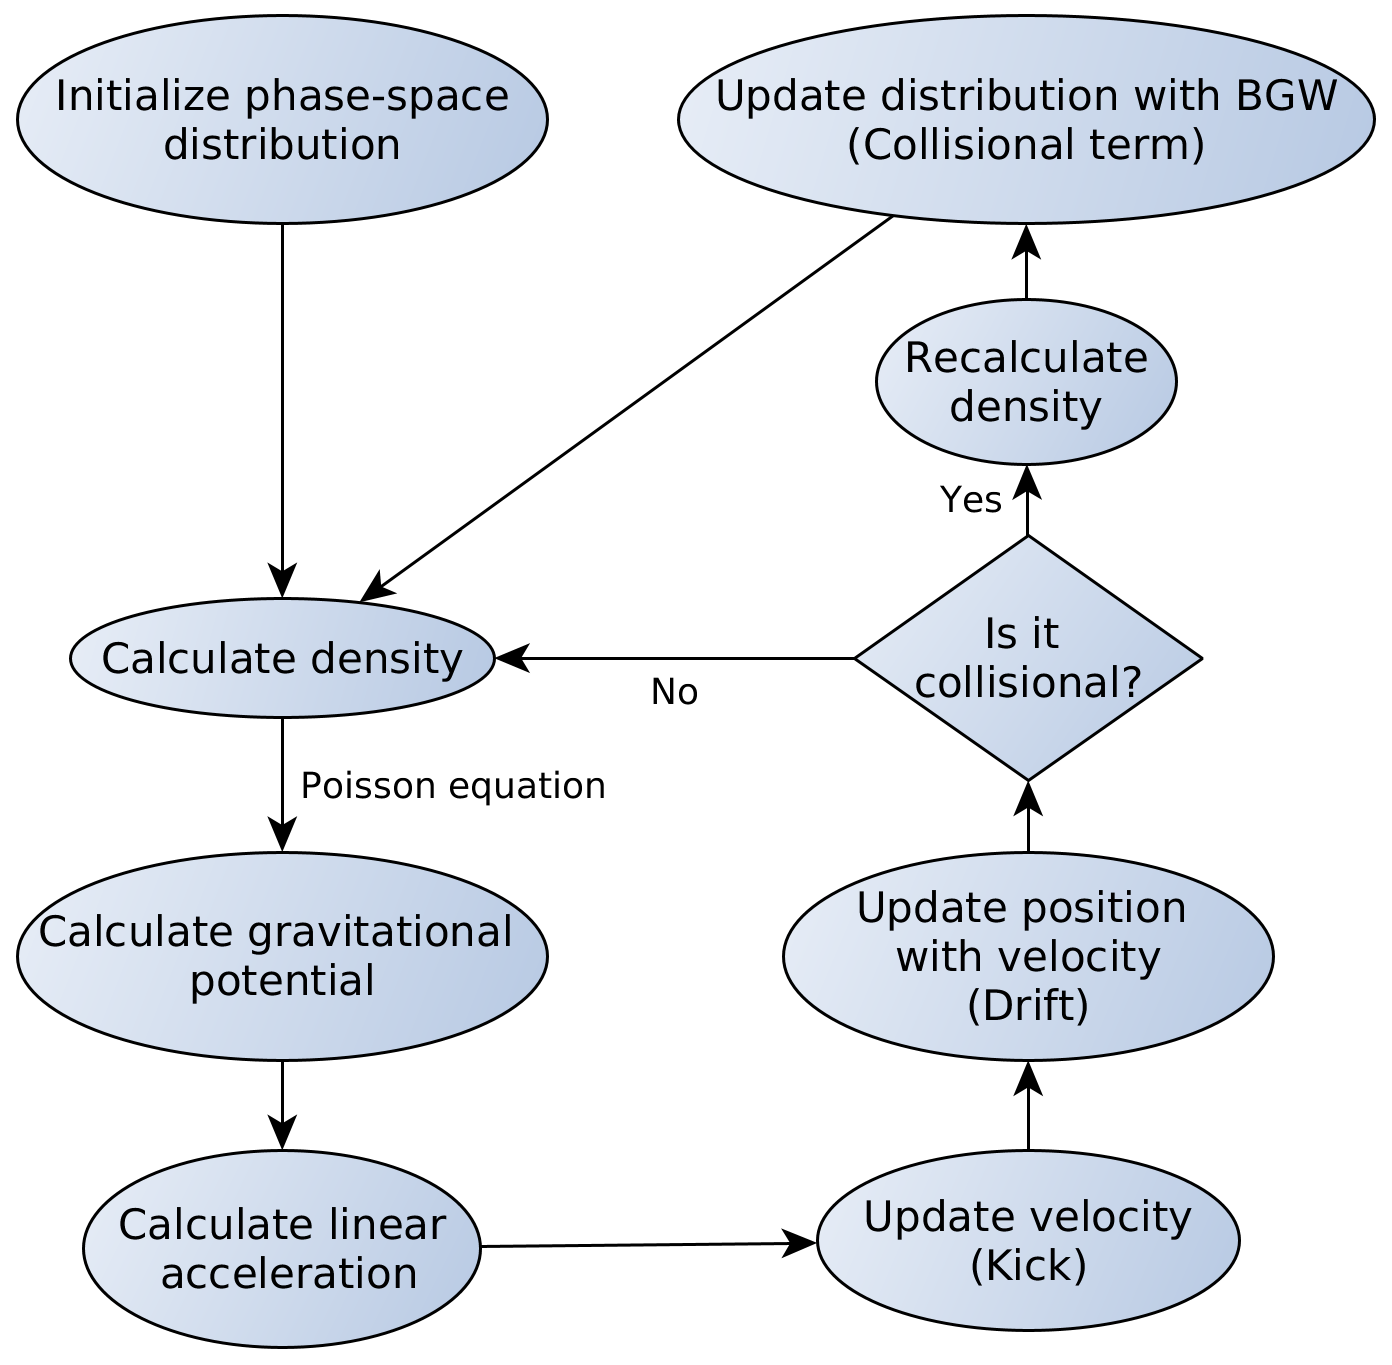
\includegraphics[scale=0.2]{imag/flowchart.png}
    \caption{Flowchat of the algorithm.}
    \label{flowchart}
\end{figure}

After having initialized the phase space, we can obtain the spatial density of matter by numerical integration in the velocity space: 
\begin{equation}
\label{defDens0}
\dens[t] = \int_{-\infty}^{\infty} \! \f[t] \, \dd \vb{v}.
\end{equation}
When evaluating in the lattice the integral becomes a sum over the entire velocity lattice:
\begin{equation}
\label{defDens}
\dens[t] = \sum_{\vb{V}_{min}}^{\vb{V}_{max}} \f[t] \, \dd \vb{v}
\end{equation}
and during initialization:
\begin{equation}
\dens[0] = \sum_{\vb{V}_{min}}^{\vb{V}_{max}} \f[0] \, \dd \vb{v}
\end{equation}
Once we have calculated the density, we solve the Poisson equation to obtain the potential due the gravitational interaction:	\cite{integerLatticeDynamics}
\begin{myequation}
\laplacian \pot = 4 \pi G \dens
\end{myequation}
%TODO:añadir \\
Where $\pot$ is the gravitational potential and $G$ is the gravitational constant.
To solve the Poisson equation we use the Fourier pseudo-spectral method, which allows for very fast numerical solutions by making use of the Fast Fourier Transform algorithm. The idea is simply to apply a Fast Fourier Transform (FFT) to the density, then solve the equation in the Fourier space, and then apply an inverse transform (IFFT). In the Fourier space the Poisson equation is given by\cite{freePoisson} \cite{computerUsingParticles}
\begin{myequation}
\lambda_{\vb{k}}^2 \hat{\Phi}(\vb{k},t) = 4 \pi G \hat{\rho}(\vb{k},t)
\end{myequation}
Where $\hat{g}(\vb{k},t)$ is the Fourier transform of $g(\vb{r},t)$, and $\lambda_{\vb{k}}$ is a constant that depends on the size of the lattice and the wave vector $\vb{k}$.
$\lambda_{\vb{k}}$ is calculated according to the approximation scheme used to solve the equation.
In the the pseudo-spectral approximation, $\lambda_{\vb{k}}$ is given by:
\begin{myequation}
\lambda_{\vb{k}}^2 = \qty(\frac{2 \pi k_x}{X_{max} - X_{min}})^2 + \qty(\frac{2 \pi k_y}{Y_{max} - Y_{min}})^2 + \qty(\frac{2 \pi k_z}{Z_{max} - Z_{min}})^2
\end{myequation}
Therefore, solving the Poisson equation in the Fourier space is reduced to simple arithmetic.
Thanks to the highly efficient implementations of the Fast Fourier Transform Algorithm available nowadays, solving the Poisson equation takes very little time and computational resources.
In this work we use the Fastest Fourier Transform of the West\cite{FFTW} subroutine to handle the Fast Fourier Transforms.

Once we have calculated the potential, obtaining the acceleration is straight-forward:
\begin{myequation}
\acce = -\grad \pot
\end{myequation}
Which, in the context of the lattice can be easily calculated with a central difference numerical derivative.

Now, in order to update the phase space, we must first define the time interval to simulate: we name $N_t$ the number of time \emph{instants} to simulate and $\dd t$ the length of each of such instants.
After calculating the acceleration and defining $\dd t$, we can update our phase space.
As mentioned in section \ref{boltz}, the subtlety here is that we will only use integer arithmetic, which means that we do not exactly care about the change in velocity during a time $\dd t$, but for how many cells in the phase space lattice that change represents. This is modeled by:
\begin{equation}
\vb{v}_{n+1} = \vb{v}_n + \toInt{\vb{a}_n \dd t}
\end{equation}%\\%\vspace{5mm}\\
With $\toInt{x}$ representing the operator \tqt{to nearest integer}, so that $\vb{v}$ and $\toInt{\vb{a} \dd t}$ are vectors of integers and $n$ represents the time instant. The update of the velocity is known as \tqt{kick}. Analogously, the update of the position is known as \tqt{drift}, and is given by:
\begin{myequation}
\vb{r}_{n+1} = \vb{r}_n + \toInt{\vb{v}_n \dd t}
\end{myequation}\\
The use of only integer arithmetics allows for the elimination of the rounding error but introduces lattice noise. Regardless, this method creates a one to one map with the continous solution\cite{franco} \cite{integerLatticeDynamics}.\\ \\ 
\vspace{-1mm} The \tqt{kick} and \tqt{drift} together are known as the \tqt{Streaming} step, and it represents the classical movement of particles under a potential but without considering the collision of particles. 
If we want a collisionless simulation, we can just calculate again the density and continue the algorithm from there. If we want a collisional simulation, we must define a collisional step.

\section{The Collisional Step}
\label{metodologiaBGK}
As previously mentioned, solving the collisional integral $C[f]$ is not a straight-forward task, as it depends on the modeling of the short range interactions that we decide to assign to the dark matter particle.
Given that the short range interactions of dark matter are unknown, we avoid using an specific description of the microscopic interactions and choose to use a mesoscopic approach instead, as discussed in section \ref{bgk}. The BGK collisional operator is given by:
\begin{equation}
C[f] = -\frac{1}{\tau}(\f - f_e(\rv))
\end{equation}
Which in the context of the direct integration scheme used in the simulation becomes:
\begin{equation}
f(\vb{r} + \vb{v} \dd t,\vb{v},t) = \f - \frac{\dd t}{\tau}(\f - f_e(\rv))
\end{equation}\\
The idea behind this approach is to recover the macroscopic properties of the fluid without committing to a particular microscopic description. In this scenario, the macroscopic effects of the collisions is a local relaxation towards equilibrium, which the BKG operator models using a relaxation time $\tau$ and a local equilibrium distribution $f_e(\rv)$. 

We implement the collisional operator as a collisional step after the streaming step, in which the system performs a relaxation with characteristic (relaxation) time $\tau$ towards the local equilibrium distribution $f_e(\rv)$. 
It is important to note that the BGK collisional operator is a \emph{scattering} operator and does not consider annihilation or creation of particles. 

After defining the collisional term, we have to choose a distribution function $f_e(\rv)$. We claim that the phase space distribution relaxes towards local equilibrium, which means a displacement in the phase space and not the introduction or annihilation of mass.
Therefore, the equilibrium distribution must be perfectly \emph{normalized}  in order to enforce particle number conservation. We normalize the equilibrium distribution by using macroscopic quantities obtained through numerical integration of the velocity part of the phase space.
This macroscopic quantities are: the spatial density $\dens$, the macroscopic velocity $\vb{u}(\rv)$ and the internal energy $e(\rv)$.

The volumetric density is the same density we have been using so far defined by the integral of equation \ref{defDens0}. The macroscopic velocity $\vb{u}(\rv)$ is defined by the integral:
\begin{equation}
\vb{u}(\rv) = \int_{-\infty}^{\infty} \! \f[t] \, \vb{v}  \dd \vb{v}.
\end{equation}

When evaluating in the lattice the integral becomes:
\begin{equation}
\label{defVel0}
\vb{u} = \sum_{\vb{V}_{min}}^{\vb{V}_{max}} \f[t] \,  \vb{v} \dd \vb{v}
\end{equation}
And the internal energy is defined by the integral:
\begin{equation}
e(\rv) = \frac{1}{2} \int_{-\infty}^{\infty} \! \f[t] \, (\vb{v} -\vb{u})^2 \dd \vb{v}.
\end{equation}
Which also becomes a sum when evaluating in the lattice:
\begin{equation}
\label{defEn0}
e(\rv) = \frac{1}{2} \sum_{\vb{V}_{min}}^{\vb{V}_{max}} \f[t] \,  (\vb{v} -\vb{u})^2 \dd \vb{v}
\end{equation}\vspace{2mm} 

Note that we are not including explicitly the mass of the dark matter particle in this integrals because it has already been included in the definition of the phase space.

Now that we have well defined macroscopic variables, we can proceed to choose an equilibrium distribution. Such distribution must obey the following condition:
\begin{equation}
C[f_e] = 0
\end{equation}
Which simply means that if the system is already in local equilibrium, then there is no relaxation. This condition can also be stated as \tqt{the equilibrium function must be a collisional invariant}. In order for $f_e(\rv)$ to be a collisional invariant, it must be build with variables that are also collisional invariant. Fortunately, the macroscopic variables already defined in this chapter are also collisional invariants, and so, we can use them to build equilibrium distributions. The idea behind normalization is to obtain the same macroscopic variables when integrating over $f_e(\rv)$ instead of $\f$.  In this work we use distributions based on the Maxwell-Boltzmann velocity distribution. Alternative equilibrium distributions functions can be considered and may be of interest, but they are beyond the scope of this work. In particular, quantum Maxwellians may be used to include annihilation and creation of particles, and the effects of Bose-Einstein, Fermi-Dirac statistics\cite{2010arXiv1009.3352F}.

The equilibrium function to use is a classical Maxwellian properly normalized for the case of interest:
\begin{equation}
f_e(\rv) = \frac{\rho}{[2 \pi \ e(\rv) ]^{D/2}} \exp[-\frac{(\vb{v}-\vb{u})^2}{2 \ e(\rv)}]
\end{equation}
Where $D$ is the number of spatial dimensions. For example, if the system is a three dimensional dark matter halo, then D will be equal to three.
The Maxwell distribution was originally used to describe the probability distribution of the velocity in a gas under kinetic theory assumptions. Here, we assume collisions as a phenomena that happens instantly. During the time in between, the mechanics of the system are governed by the self-gravitational potential. Therefore, the Maxwell distribution is a good ansatz for the collisional equilibrium distribution function $f_e(\rv)$. \\
Finally, the only thing left to choose is a relaxation time. As in classic kinetic theory, our relaxation time will be given by: 
\begin{equation}
\tau = \frac{1}{n <\sigma v>}
\end{equation}
In terms of the matter density instead of particle number:
\begin{equation}
\tau = \frac{m}{\rho <\sigma v>}
\end{equation}
With $n$ being the mean particle number in the halo, $m$ being the mass of a dark matter particle, $\rho$ being the average density of a dark matter halo and $<\sigma v>$ is the thermally averaged cross-section of the particle.\\
For this simulation we use the average \emph{matter} density of the universe, given by the most recent results of the Planck probe\cite{2018arXiv180706209P}. We are also going to use the value of $<\sigma v>$  constrained by the Bullet Cluster data \cite{2008ApJ6791173R} \cite{2017MNRAS465569R}, and for the dark particle mass we are going to use the lowest mass possible for a fermionic dark matter particle candidate \cite{mariangela}. These values are:
\begin{align}
m &= 0.7 \ \text{KeV} \\
<\sigma v> &= 3 \e{-26} \ \text{cm}^3 / \text{s}\\
\rho = \Omega_m &= 0.312  
\end{align}
The final value of $\tau$ will depend on the particular set of units used in every scenario. Alternative set of values may be used to test dark matter particle candidates.

\subsection{Parameters of the simulation}
There are still two important aspects of the simulation to be defined: the units and the boundary conditions.

To set the units we fix the value of one spatial unit ($us$), one unit of time ($ut$), and one unit of mass ($um$) of the simulation, and from there, we proceed to calculate the values of the physical constants in our units.
The physical constant of interest here is the gravitational constant, since it gives the coupling of the gravitational interaction.
We chose units to simulate a dark matter halo of dimensions akin to the halo of the some galaxies of the Local Group. Because of stability conditions, the units may differ between runs, therefore, they are specified at the beginning of each section in the next chapter.

For the boundaries we implement the following conditions:
\begin{itemize}
\item The boundaries of the spatial axes are periodic. Any portion of mass that leaves the distribution, will re enter through the opposite extreme. This condition assumes the system as periodic.
\item Every portion of mass that leaves the distribution through the velocity axes will be lost forever. That means that if a particle has a velocity higher than the extremal values of the simulation, the particles is no longer considered in the next time step. This condition is not very limiting because we have high extremal values for the velocity and dark matter is traditionally modeled as \emph{cold} or \emph{warm}.
\end{itemize}


\chapter{Results}
We wrote and ran three simulations: a  two dimensional phase space simulation (one spatial and one velocity dimension), a four dimensional phase space simulation, and a six dimensional phase space simulation. 
The first one was develop in order to reproduce the results of Philip Mocz and Sauro Succi published in 2016 \cite{integerLatticeDynamics}, and the results of Sebastian Franco published in 2017 \cite{franco}.
In addition to reproducing results, we also extended the simulation to account for a collisional operator and tested it with different initial conditions.

The four dimensional simulation was develop as a step to develop the six dimensional simulation. Developing a four dimensional simulation allows to implement and test the specifics of increasing dimensionality without much of the visualization problems that arise from a six dimensional simulation. 

The six dimensional simulation is one of the main scopes of this work. The simulation was implemented successfully, however, due to the high RAM memory requirements of the Lattice-Boltzmann method, the resolution is heavily constrained. Even using the HPC cluster avalible at \tqt{Universidad de los Andes}, the resolution of the simulation was too poor to reproduce the results from the other two simulations.

\section{The two dimensional phase space}
%\vspace{-5mm} \vspace{1mm} %descomentar
\label{primerCaso}

For the two dimensional simulation we only need two axes, which allows for very high resolution run. We used a squared grid characterized by:
\begin{align}
W_{min} &= -1\\
W_{max} &= 1\\
N_w &= 2048\\
dw &= 1/1024
\end{align}
As mentioned in section \ref{implementBoltzmann}, $W$ represents the axis (in this case $r$ or $v$), $N_w$ represents the size of the grid in the $w$ axis, $dw$ represents the size of a lattice unit in the $w$ axis and $-1$ and $1$ are the extremal values of the phase space in the $w$ axis.
We always use grid sizes of the form $N_w = 2^n$ with $n$ positive integer, because the Fast Fourier Transform algorithm performs better and faster when calculating discrete transforms of sizes $2^n \ 3^m \ 5^l$ for n,m,l positive integers.%\\ \\ 
%\vspace{-1mm}

In this section we are going to use three initial conditions:
\begin{itemize}
\item A Gaussian density profile used to test the code and introduce the behavior of the phase space density over time.
\item A Jeans instability test, in which we reproduce the spatial conditions for a periodic jeans oscillation and use a Gaussian profile for the velocity distribution. These conditions are used to reproduce the previous work aforementioned. 
\item A Bullet Cluster-like initial conditions, in which we have two Gaussian profiles (each one with its own variance and amplitude) separated by a given distance. One of the main scopes of this work is to analyze the Bullet Cluster-like system and compare the phase space evolution of the collisional case with its collisionless counterpart.
%Additionally, we are going to reproduce the behavior of the collisional baryonic gas.
\end{itemize}
\subsection{No collisional case}
We begin with the Gaussian conditions because their simplicity and ease to analyze makes them the best introductory example.
The initialization of the phase space can be seen in figure \ref{1dInit}, along with its correspondent spatial density.
After initialization we proceed to calculate the potential and the acceleration, which can be seen in figure \ref{1dInit2}.
The values used to initialize the phase space were:
\begin{align}
\sigma_r &= 0.06 \ \text{us} \\
\sigma_v &= 0.06 \ \text{us} / \text{ut} \\
A &= 40  \ \text{um}
\end{align} 
Which yields a total mass of $9 \e{9}$ M$_{\odot}$, a value in accordance with recent estimates of the total mass of the Small Magallanic Cloud \cite{2009MNRAS395342B}. 

\begin{figure}[h!]
    \centering
    %\includegraphics[width=10cm,height =7cm]{Diapositiva1.jpg}
    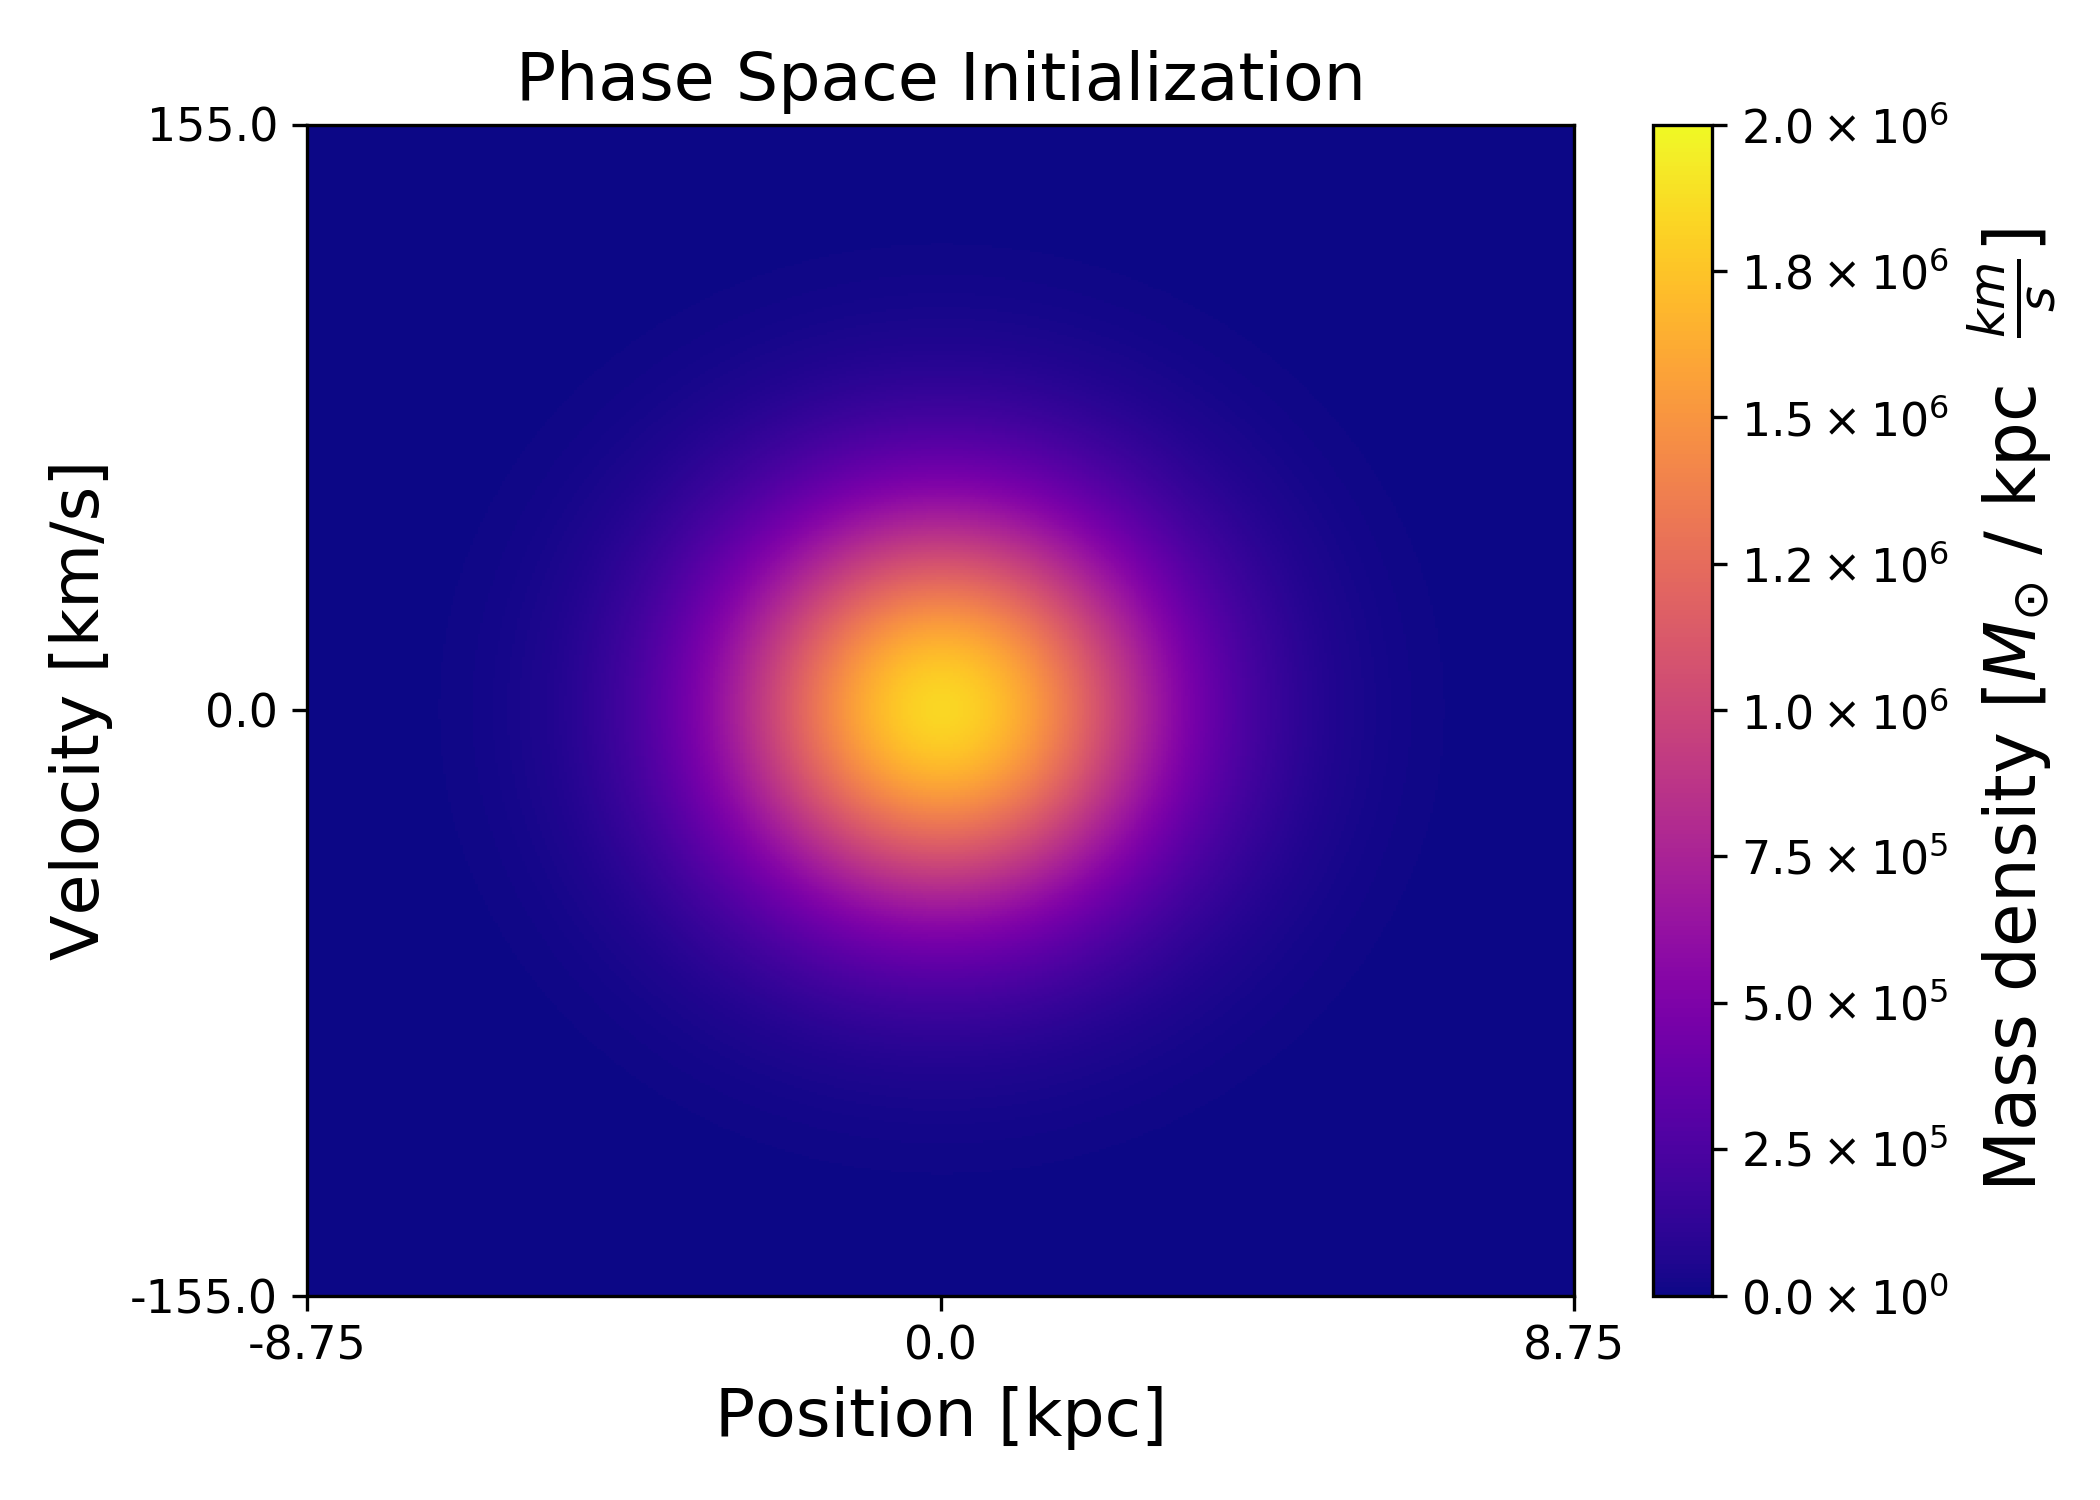
\includegraphics[scale=0.6]{imag/1dInitPS.png}
    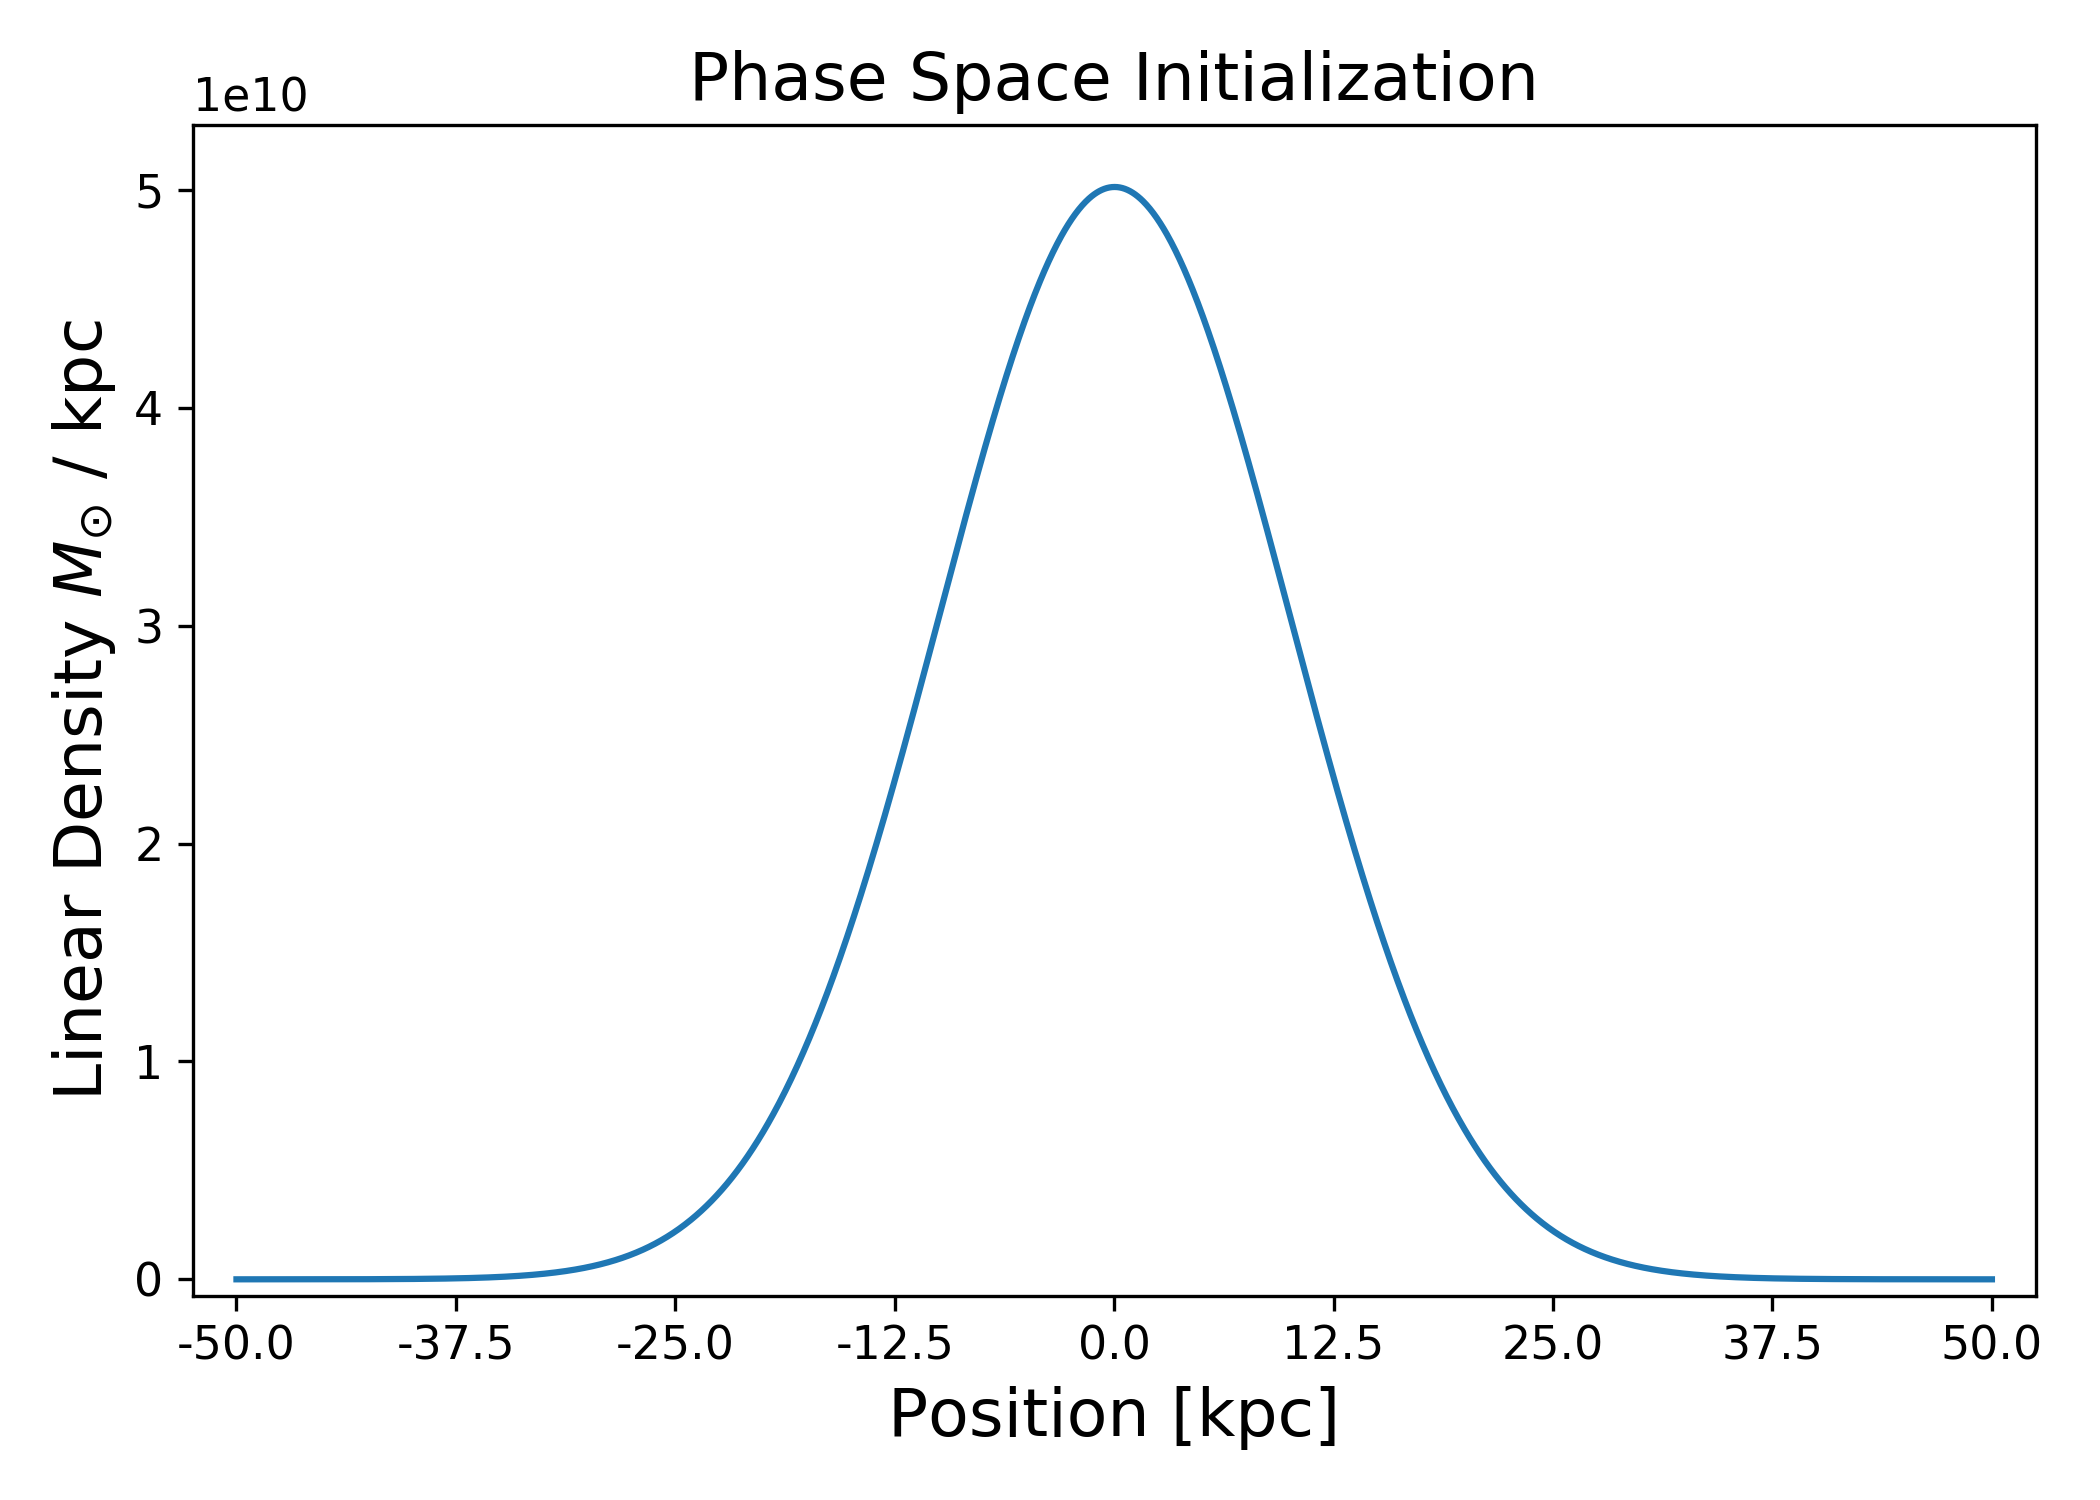
\includegraphics[scale=0.6]{imag/1dInitDens.png}
    \caption{Up: initialization of the phase space. Position is represented in the $x$ axis, and velocity in the $y$ axis of the plot. Down: the spatial density obtained through integration. }
    \label{1dInit}
\end{figure}
\newpage
\begin{figure}[h!]
    \centering
    %\includegraphics[width=10cm,height =7cm]{Diapositiva1.jpg}
    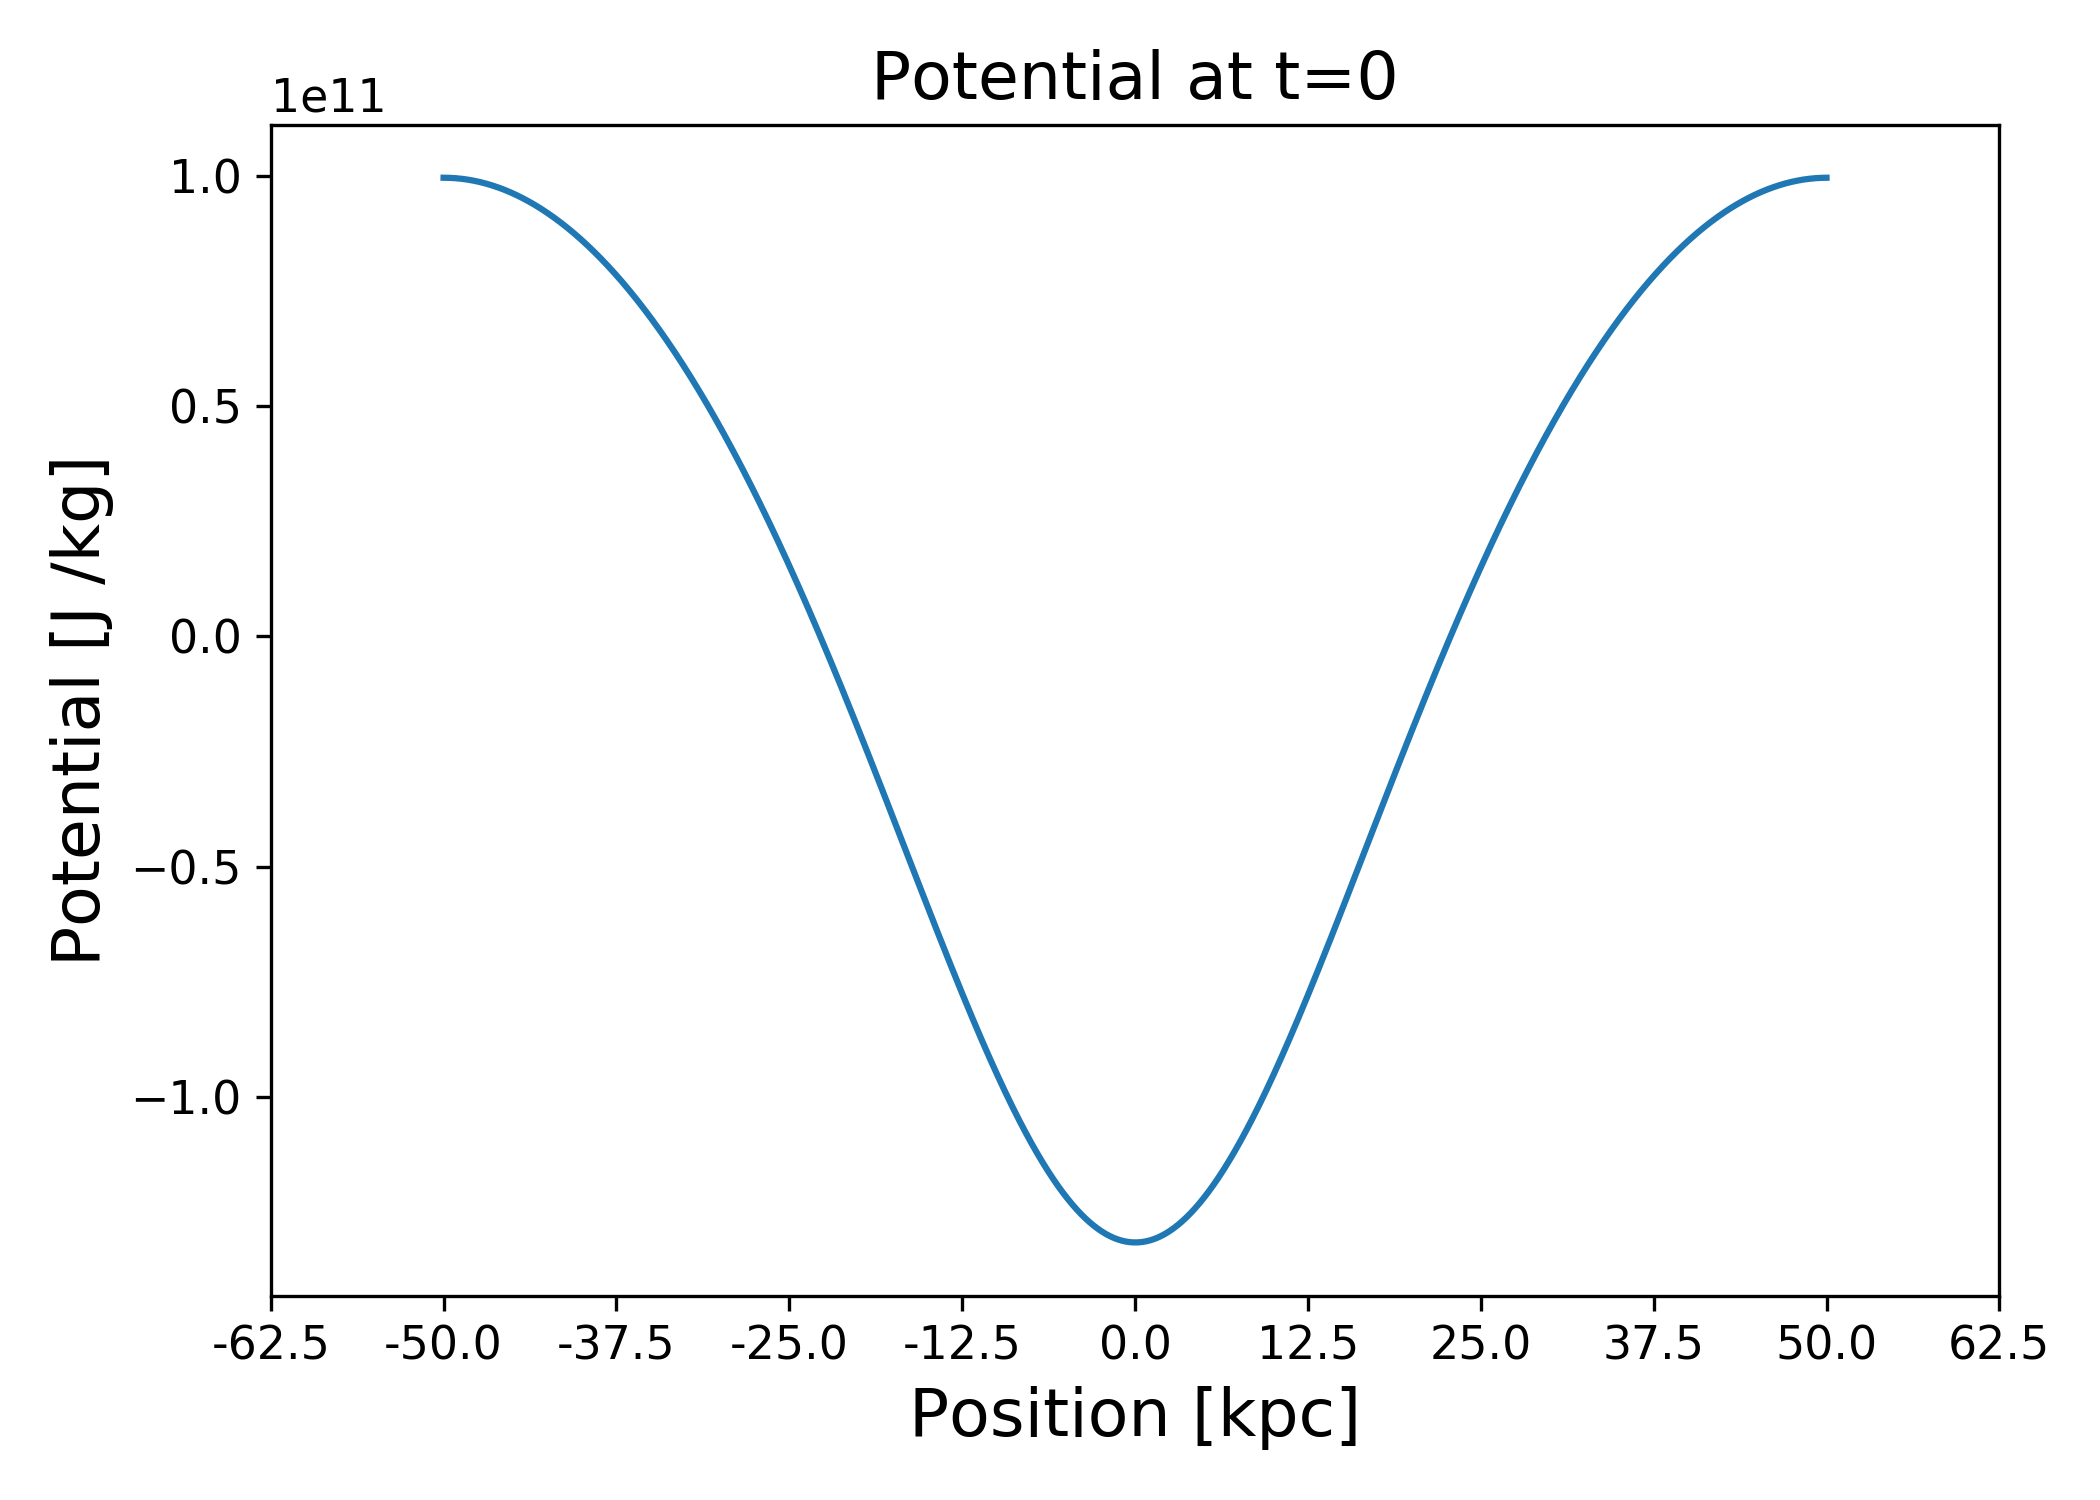
\includegraphics[scale=0.6]{imag/1dInitPot.png}
    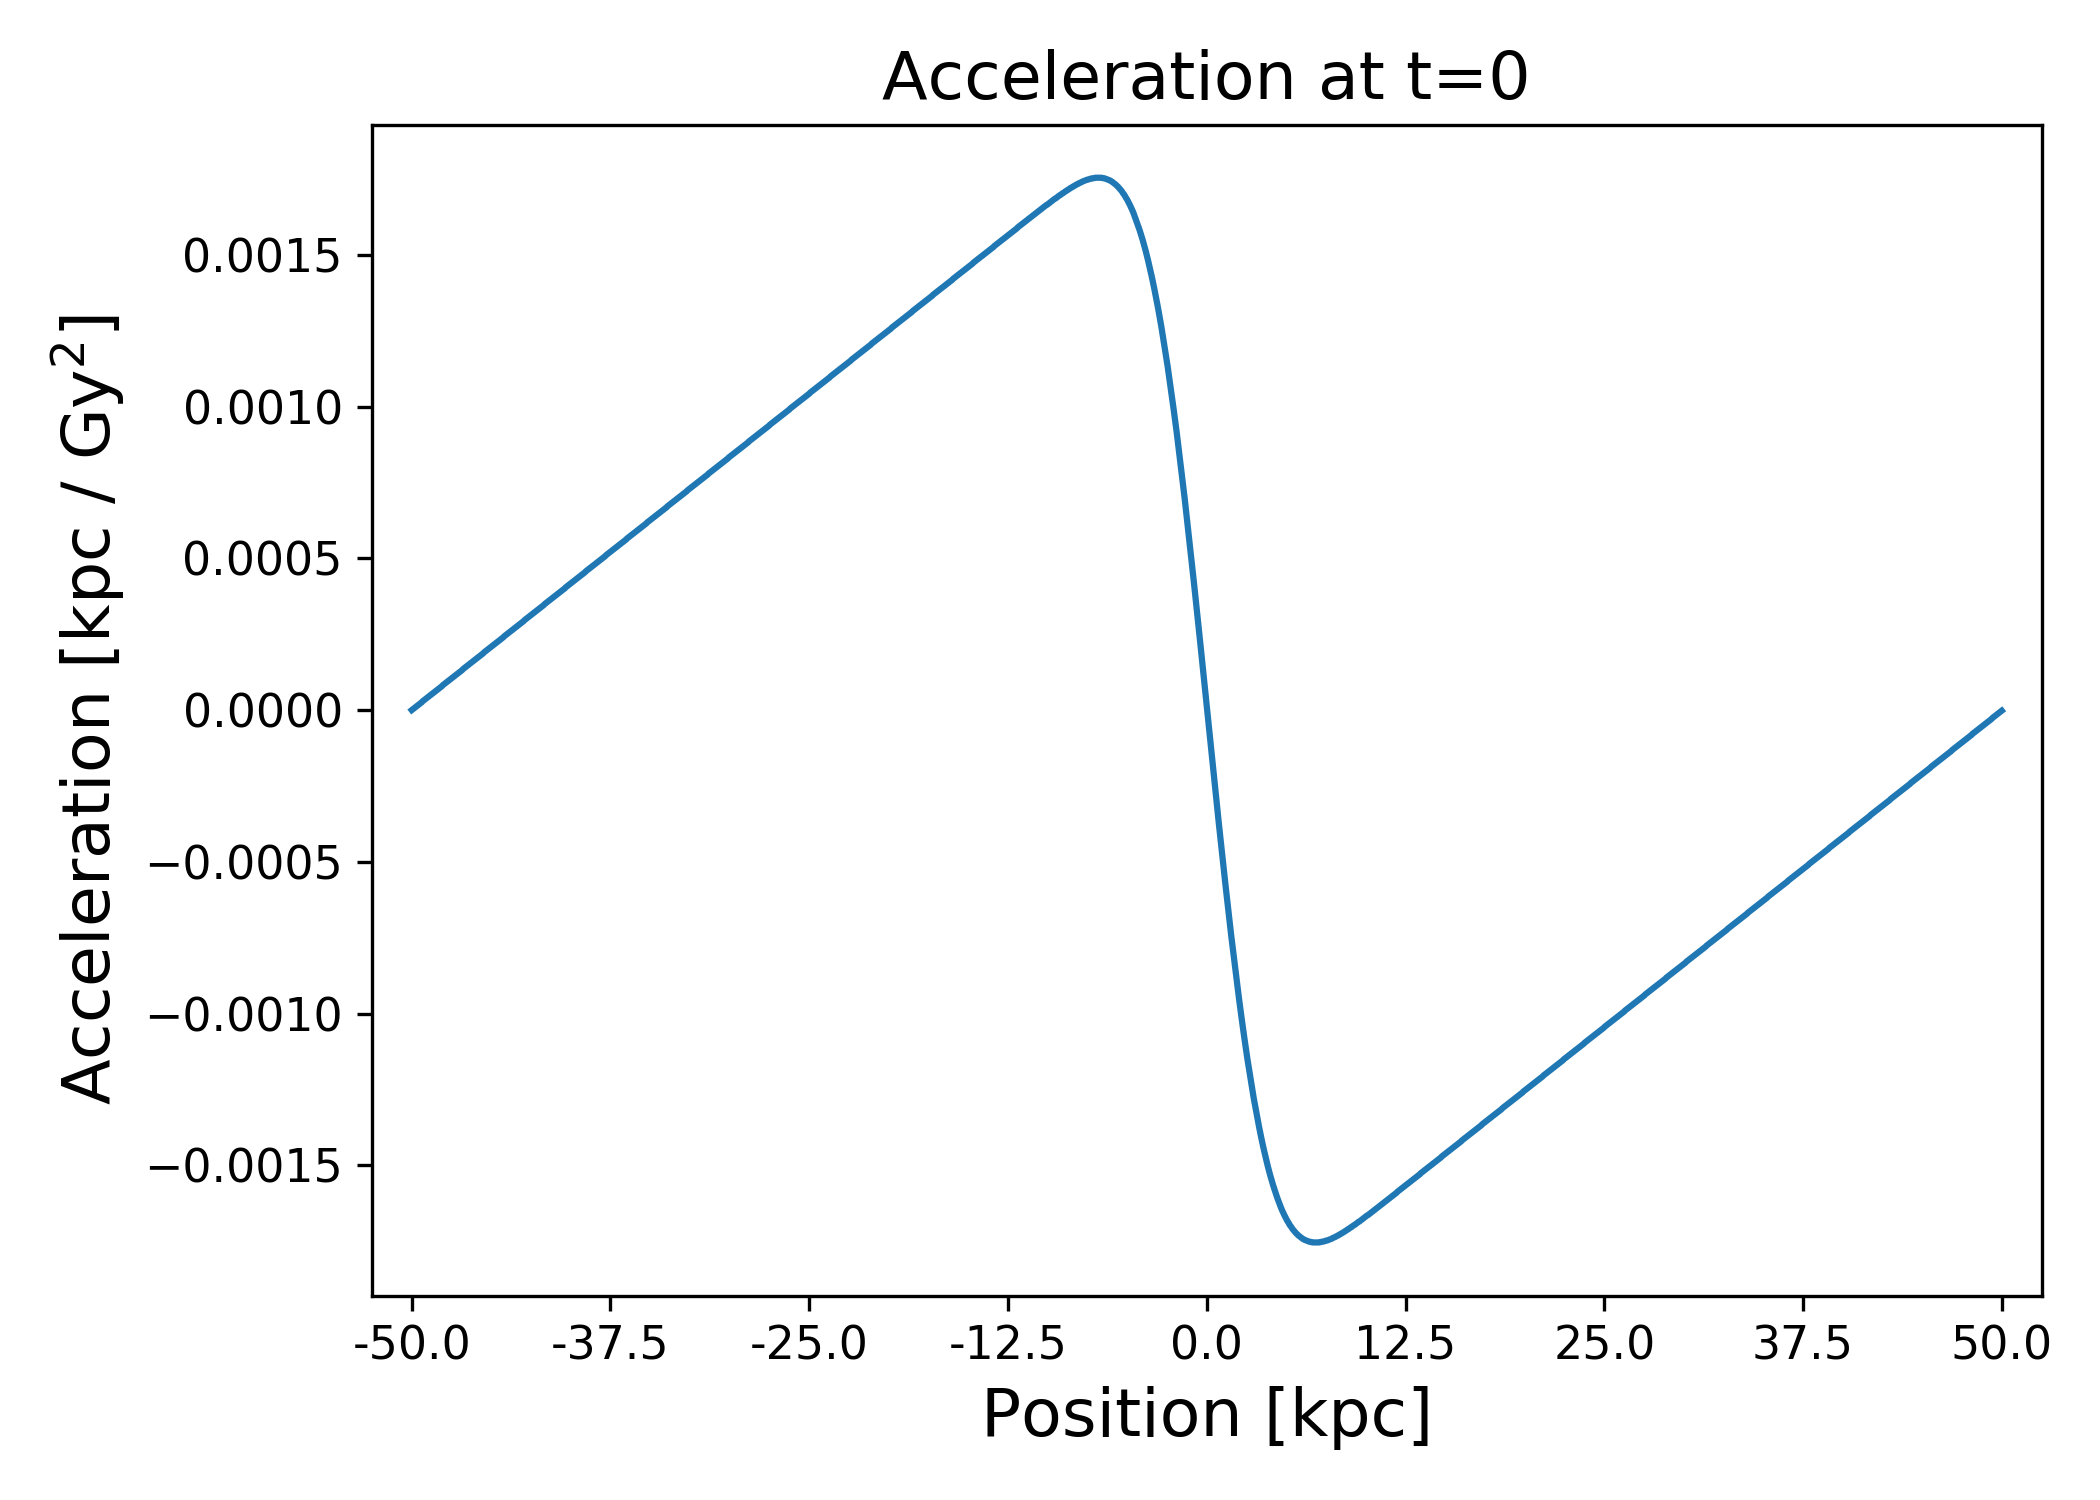
\includegraphics[scale=0.6]{imag/1dInitAcce.png}
    \caption{Up: The potential obtained by solving the Poisson equation. Given that the density was a Gaussian profile, it is no surprise that the potential is a negative Gaussian profile. Down: The acceleration obtain by numerical derivation of the potential.}
    \label{1dInit2}
\end{figure}

To test the simulation we reproduce previous work in the collisionless case.
To do so we run the simulation and check upon the behavior of the phase space density, the spatial density, the potential and the acceleration.
In the phase space grid, we expect the cells with positive velocity to move to the right side of the plot, but, as they move to the right they are also being attracted towards the left because of the symmetry of the initial conditions. Therefore, the cells with positive velocity will move towards the inferior-right side of the plot, while cells with negative velocity will move towards the upper left side of the phase space.

\begin{figure}[h!]
    \centering
    %\includegraphics[width=10cm,height =7cm]{Diapositiva1.jpg}
    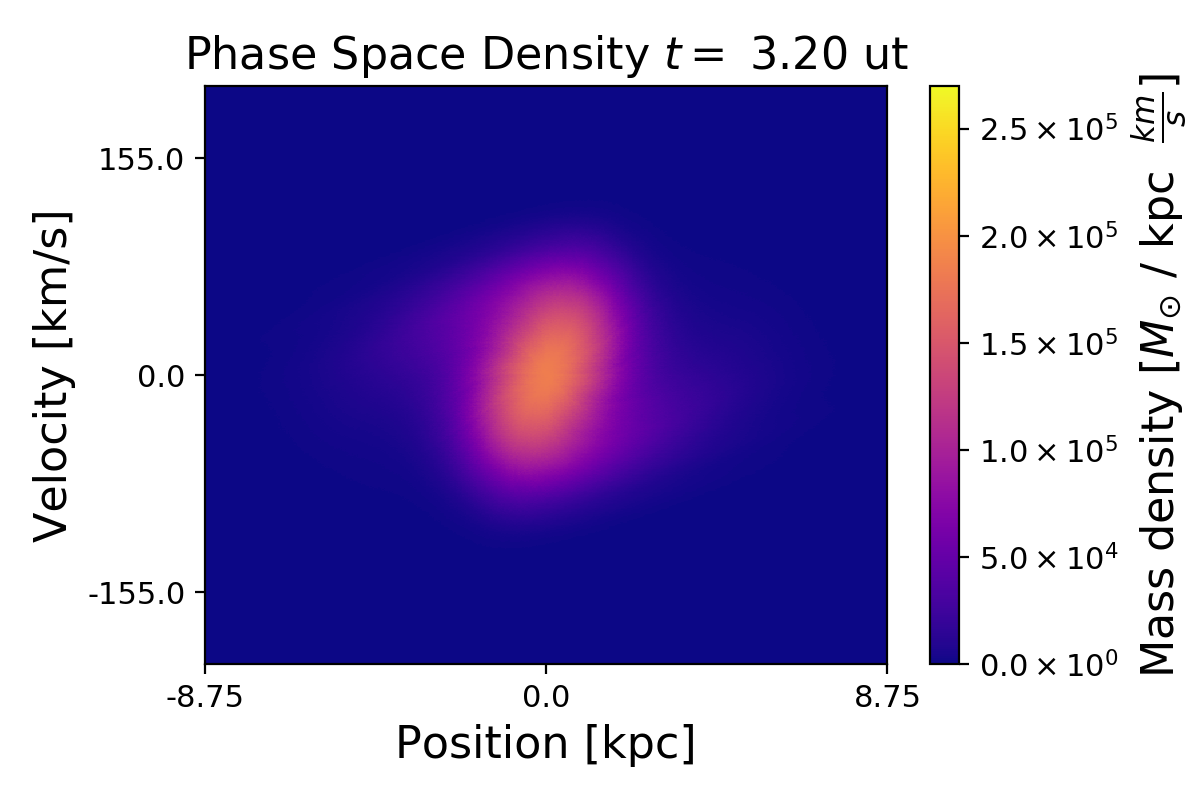
\includegraphics[scale=0.45]{imag/gauss8.png}
    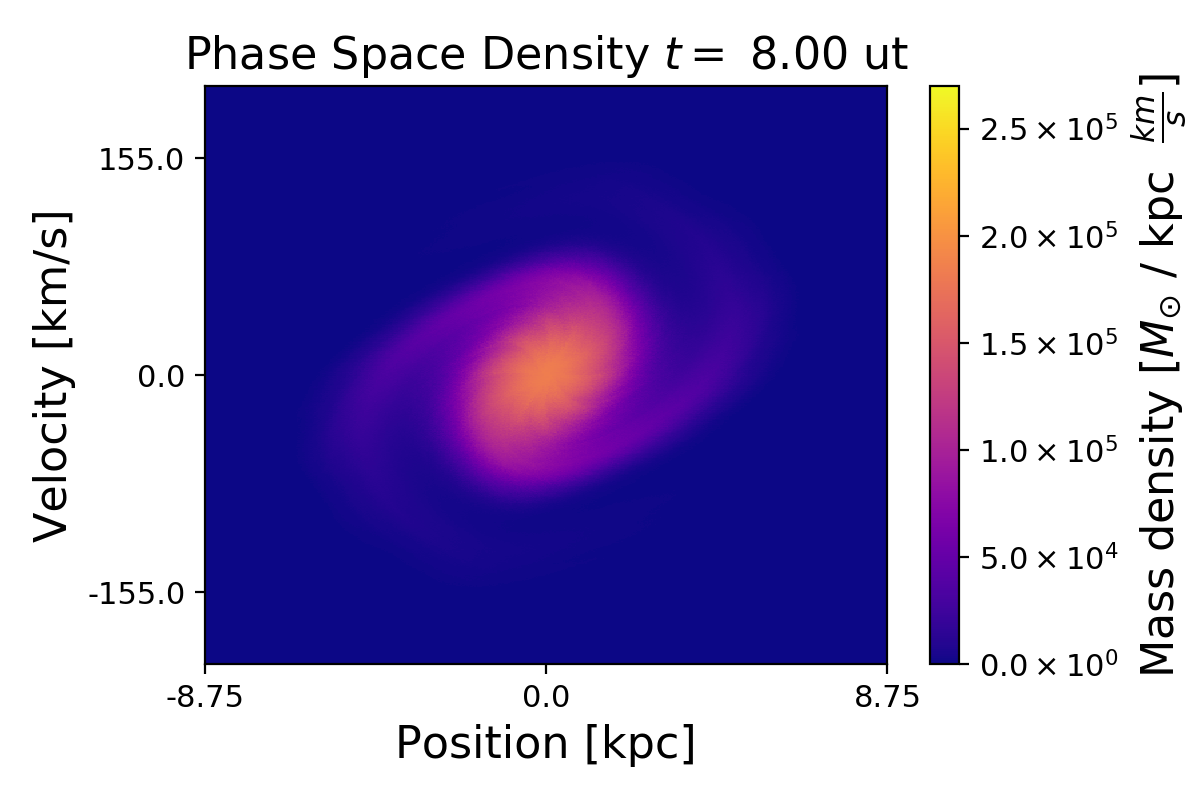
\includegraphics[scale=0.45]{imag/gauss20.png}
    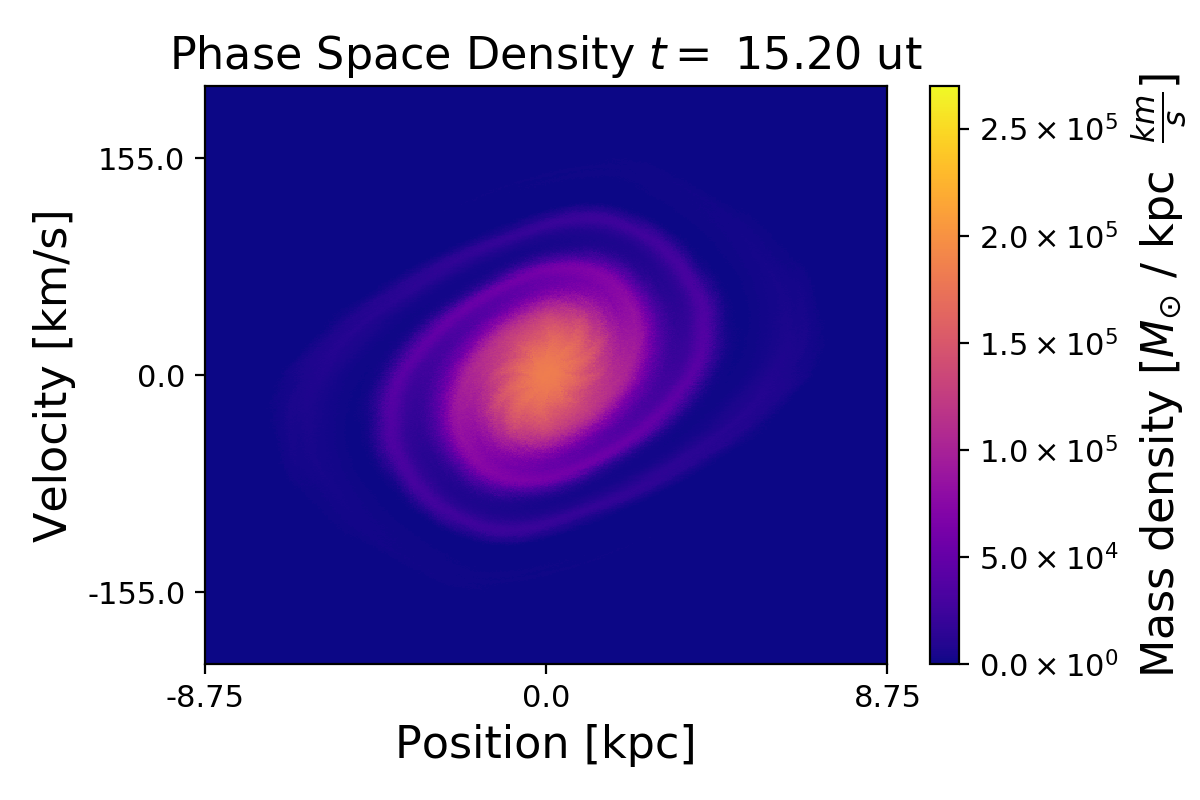
\includegraphics[scale=0.45]{imag/gauss38.png}
    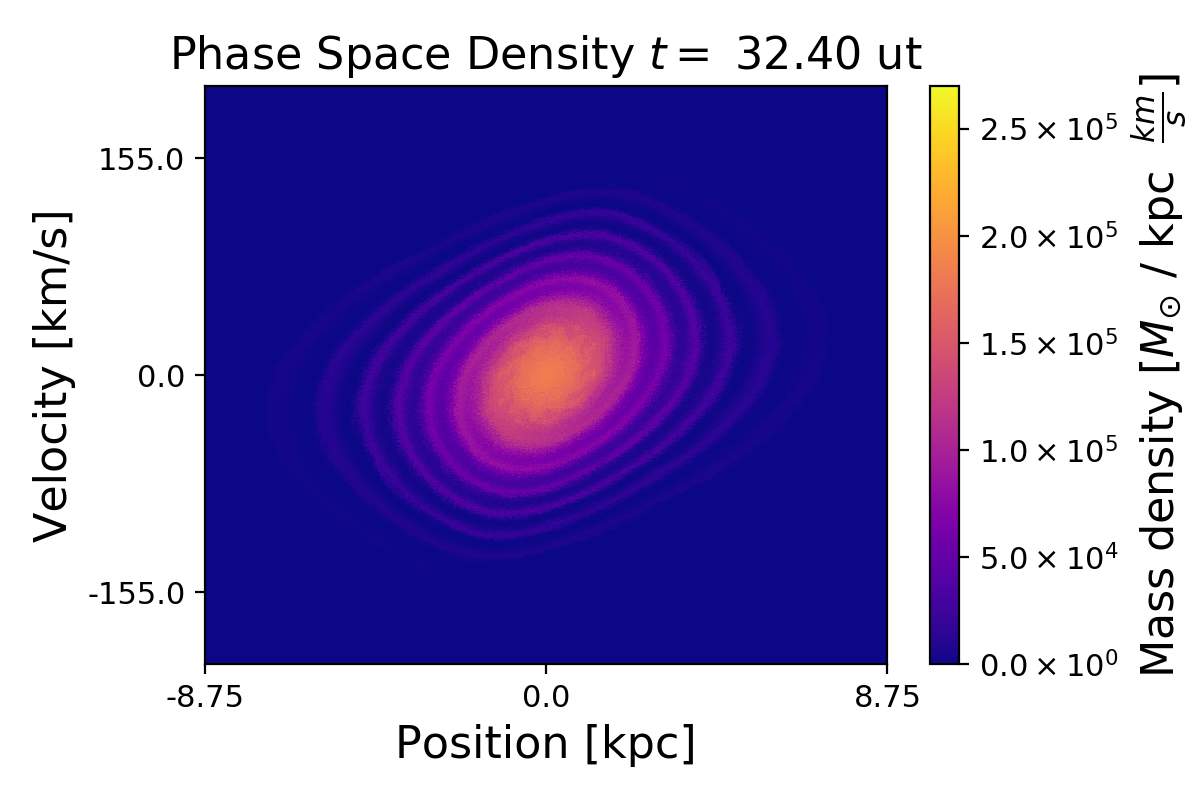
\includegraphics[scale=0.45]{imag/gauss81.png}
    \caption{Upper left: Phase space 154 million years after initialization. Upper right: Phase space 484 million years after initialization. Bottom left: Phase space 881 million years after initialization. Bottom right: Phase space 1983 million years after initialization. It is evident that the phase space behaves as a clockwise rotating spiral.}
    \label{1dphase}
\end{figure}


This behavior is in complete accordance with previous work and can be seen in figure \ref{1dphase}, where we plot different time instants chosen to display the clockwise spiral of the phase space evolution.

To visualize the linear density, we plot density vs position. We observe an initial increase in the height of the central peak and then little bumps trying to abandon the central distribution as they are gravitationally pulled back before crossing the spatial boundaries of the lattice. The bumps are simply the tails of the velocity distribution. This behavior can be seen in figure \ref{1dDens}




\begin{figure}[h!]
    \centering
    %\includegraphics[width=10cm,height =7cm]{Diapositiva1.jpg}
    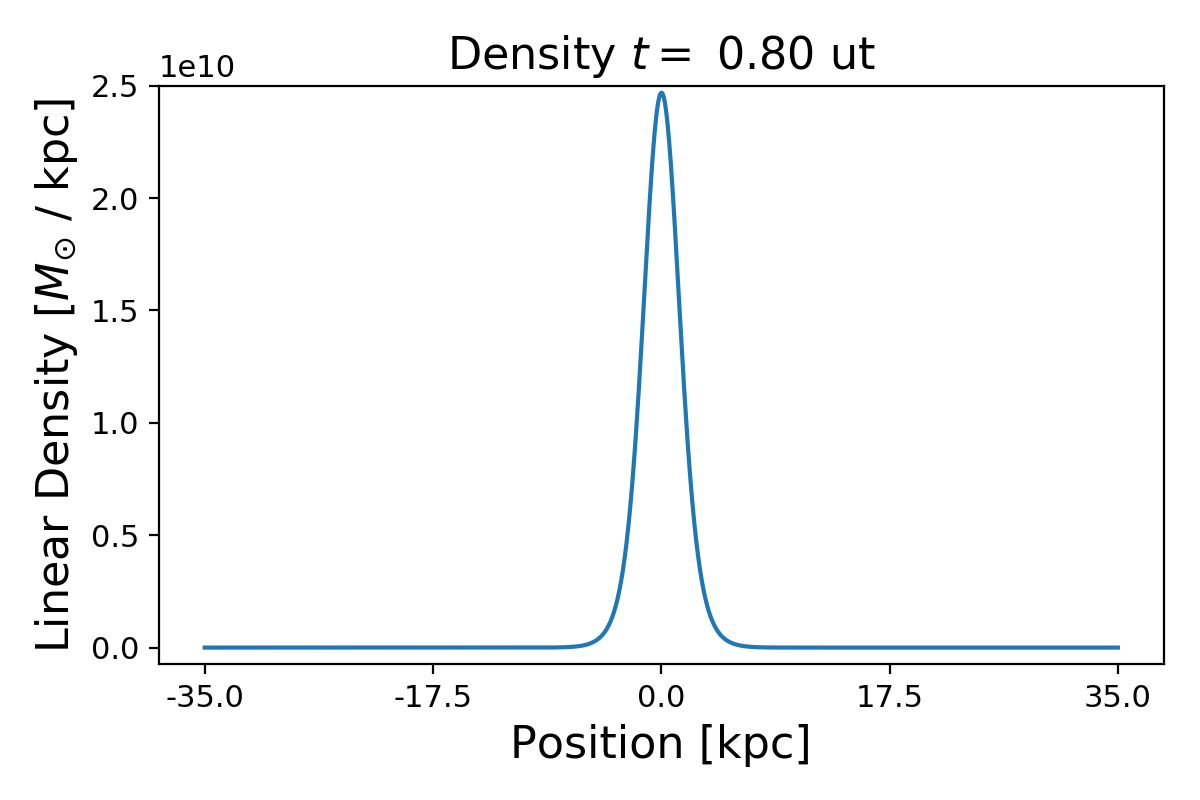
\includegraphics[scale=0.45]{imag/gaussD2.png}
    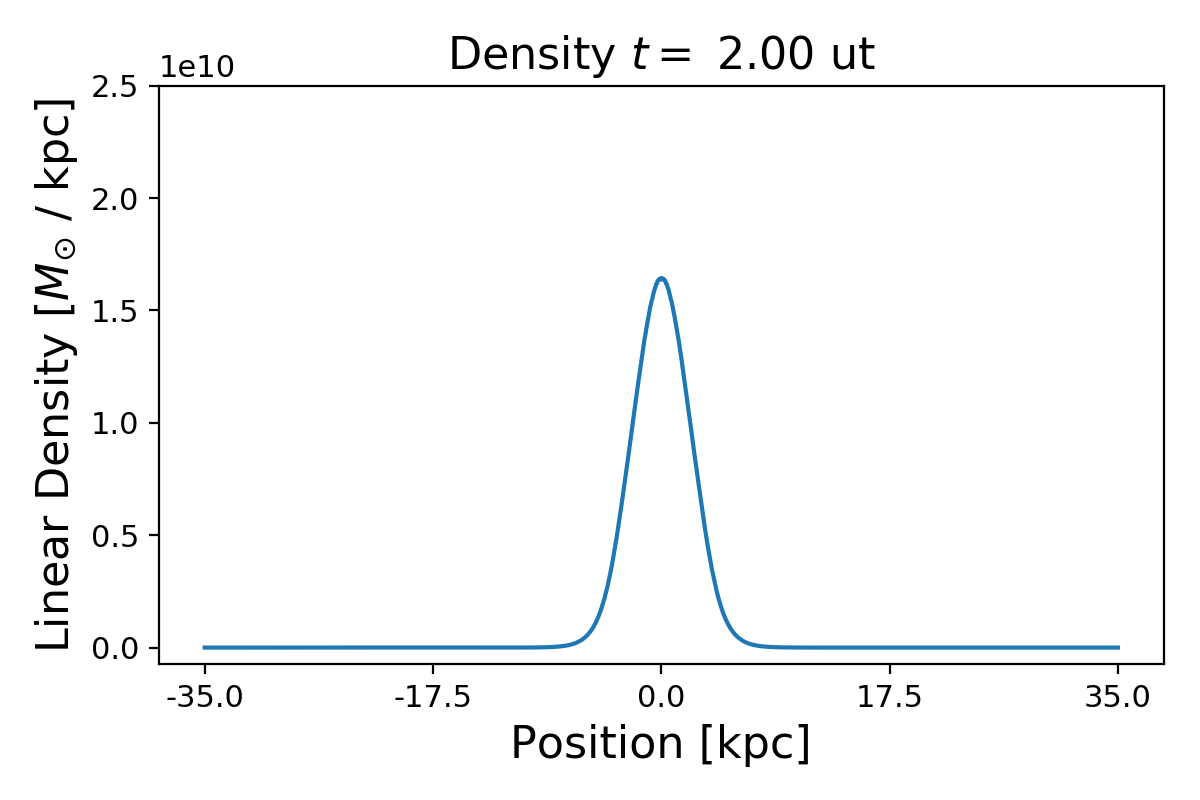
\includegraphics[scale=0.45]{imag/gaussD5.png}
    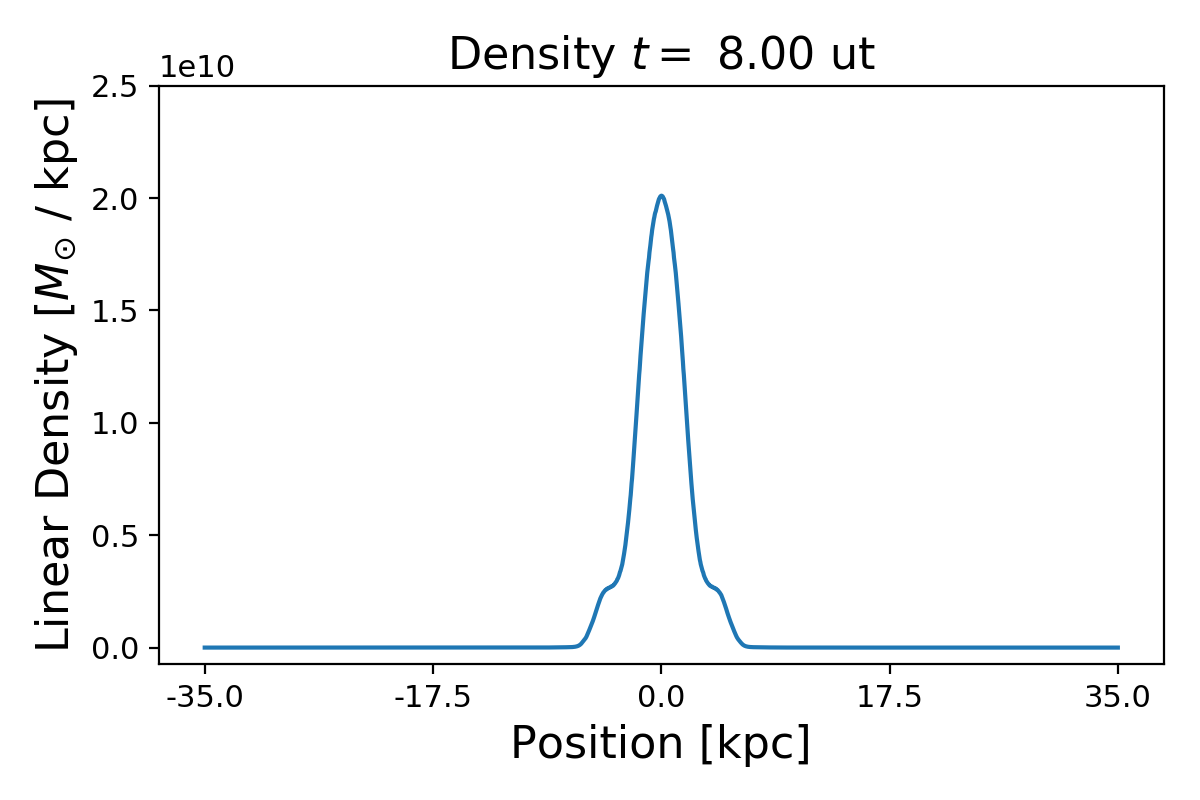
\includegraphics[scale=0.45]{imag/gaussD20.png}
    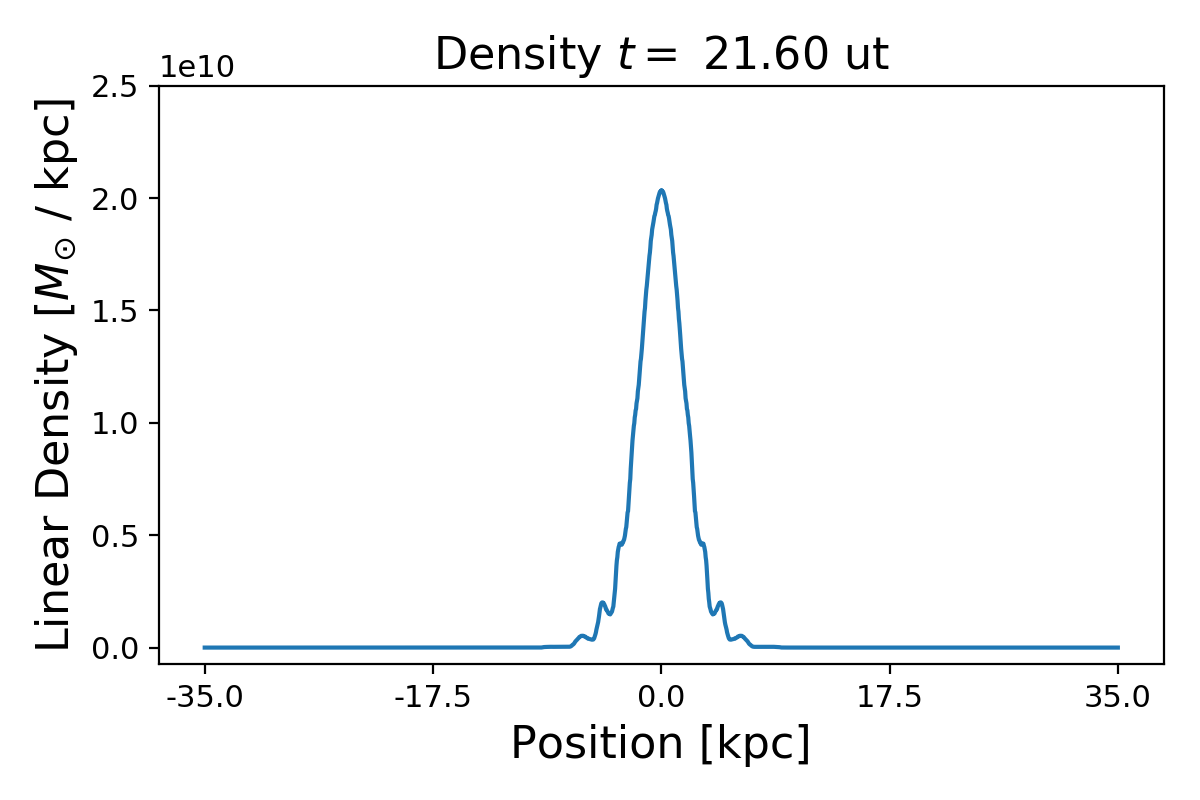
\includegraphics[scale=0.45]{imag/gaussD54.png}
    \caption{Upper left: linear density with its central peak at maximum height. Upper right: linear density with its peak at a local minima after having reached maximum height . Bottom left: little bumps can be seen at the tails of the distribution. Bottom right: the tails of the distribution are completely bumpy. These bumps are the same arms observed in the phase space.}
    \label{1dDens}
\end{figure}

In addition to the Gaussian initial conditions, we reproduced the Jeans instability, which was also tested in previous work. In this scenario, the Jeans instability is given by:
\begin{equation}
f(r,v,0) = \frac{\bar{\rho}}{(2 \pi \sigma^2)^{1/2}} \exp(-\frac{v^2}{2 \sigma^2}) (1 + A \cos(kr))
\end{equation}\\
\vspace{-1mm}Such that $\bar{\rho}$ is the average phase density of the system, $\sigma^2$ is the variance of the velocity Gaussian profile, $A$ is the amplitude of the density fluctuation and $k$ is the wave number of the density fluctuation. The values used were:
\begin{align}
\bar{\rho} &= 10 \  \text{um} \ \text{us}^{-1} \ (\text{us/ut})^{-1} \\
\sigma &= 0.1 \ \text{us/ut} \\
A &= 0.9999 \\
k &= 2 \pi \ \text{us}^{-1}
\end{align}
For which the phase space behaved like three successive Gaussian profiles, that is because we met the Jeans instability criteria. Otherwise, the distributions would have collapsed to form just one big halo. This result were also compatible with previous work published on one dimensional collisionless dark matter fluids. The evolution of the Jeans instability phase space can be seen in figure \ref{1dJeans}.\\
\\The last set of initial conditions is the Bullet Cluster-like scenario, in which two Gaussian distributions of mass collide due to their gravitational interaction, each Gaussian having its own variance and amplitude.
In the real Bullet Cluster one of the clusters was heavier than the other, therefore, we also fix one halo heavier in our simulation.

\begin{figure}[h!]
    \centering
    %\includegraphics[width=10cm,height =7cm]{Diapositiva1.jpg}
    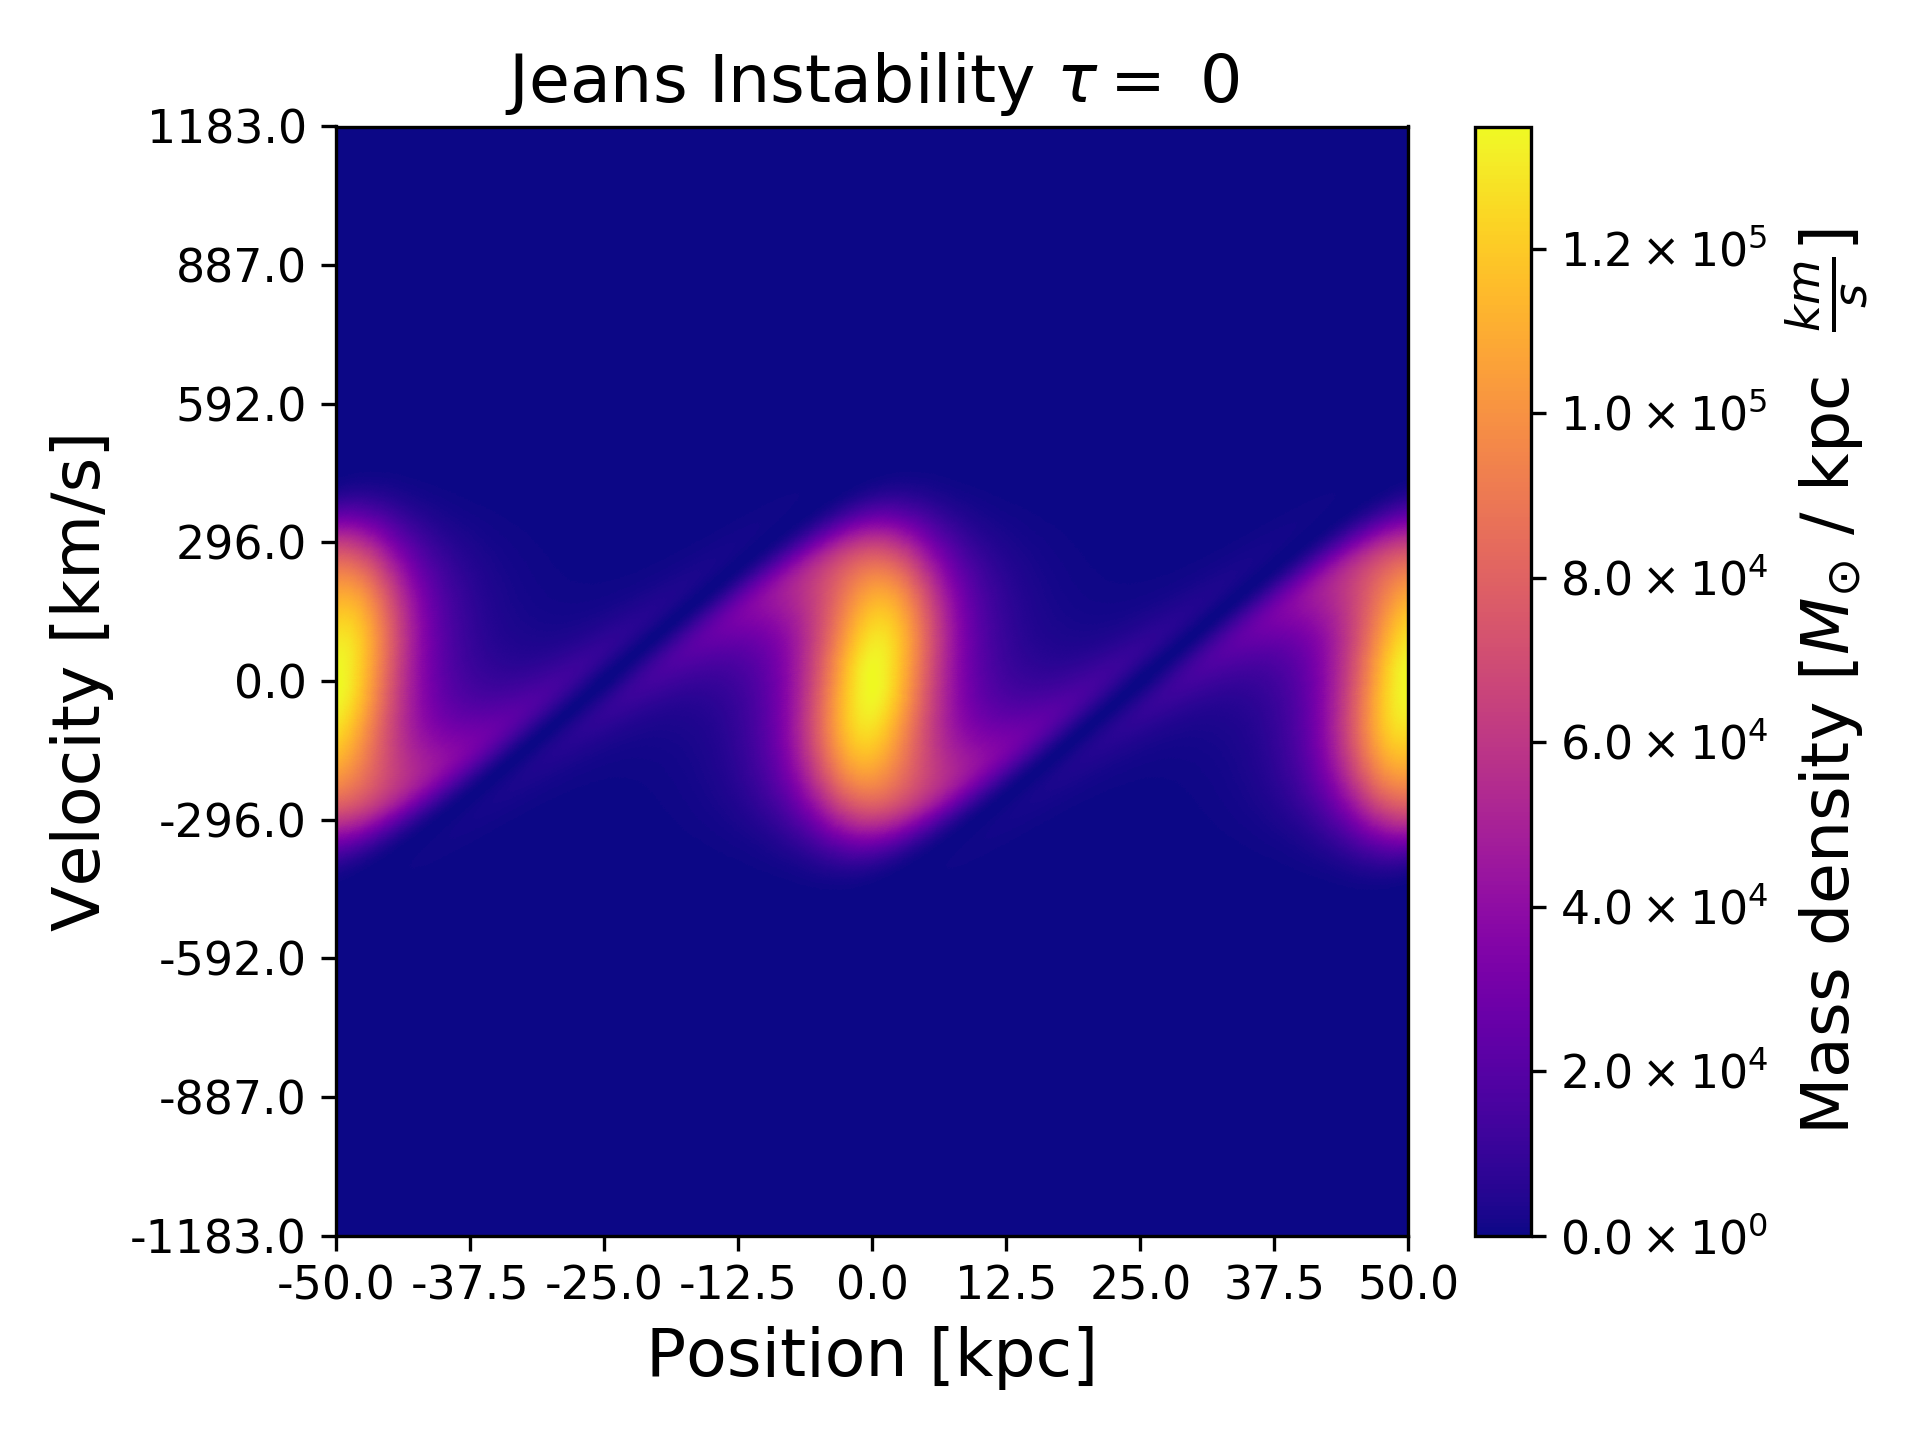
\includegraphics[scale=0.45]{imag/jeans7.png}
    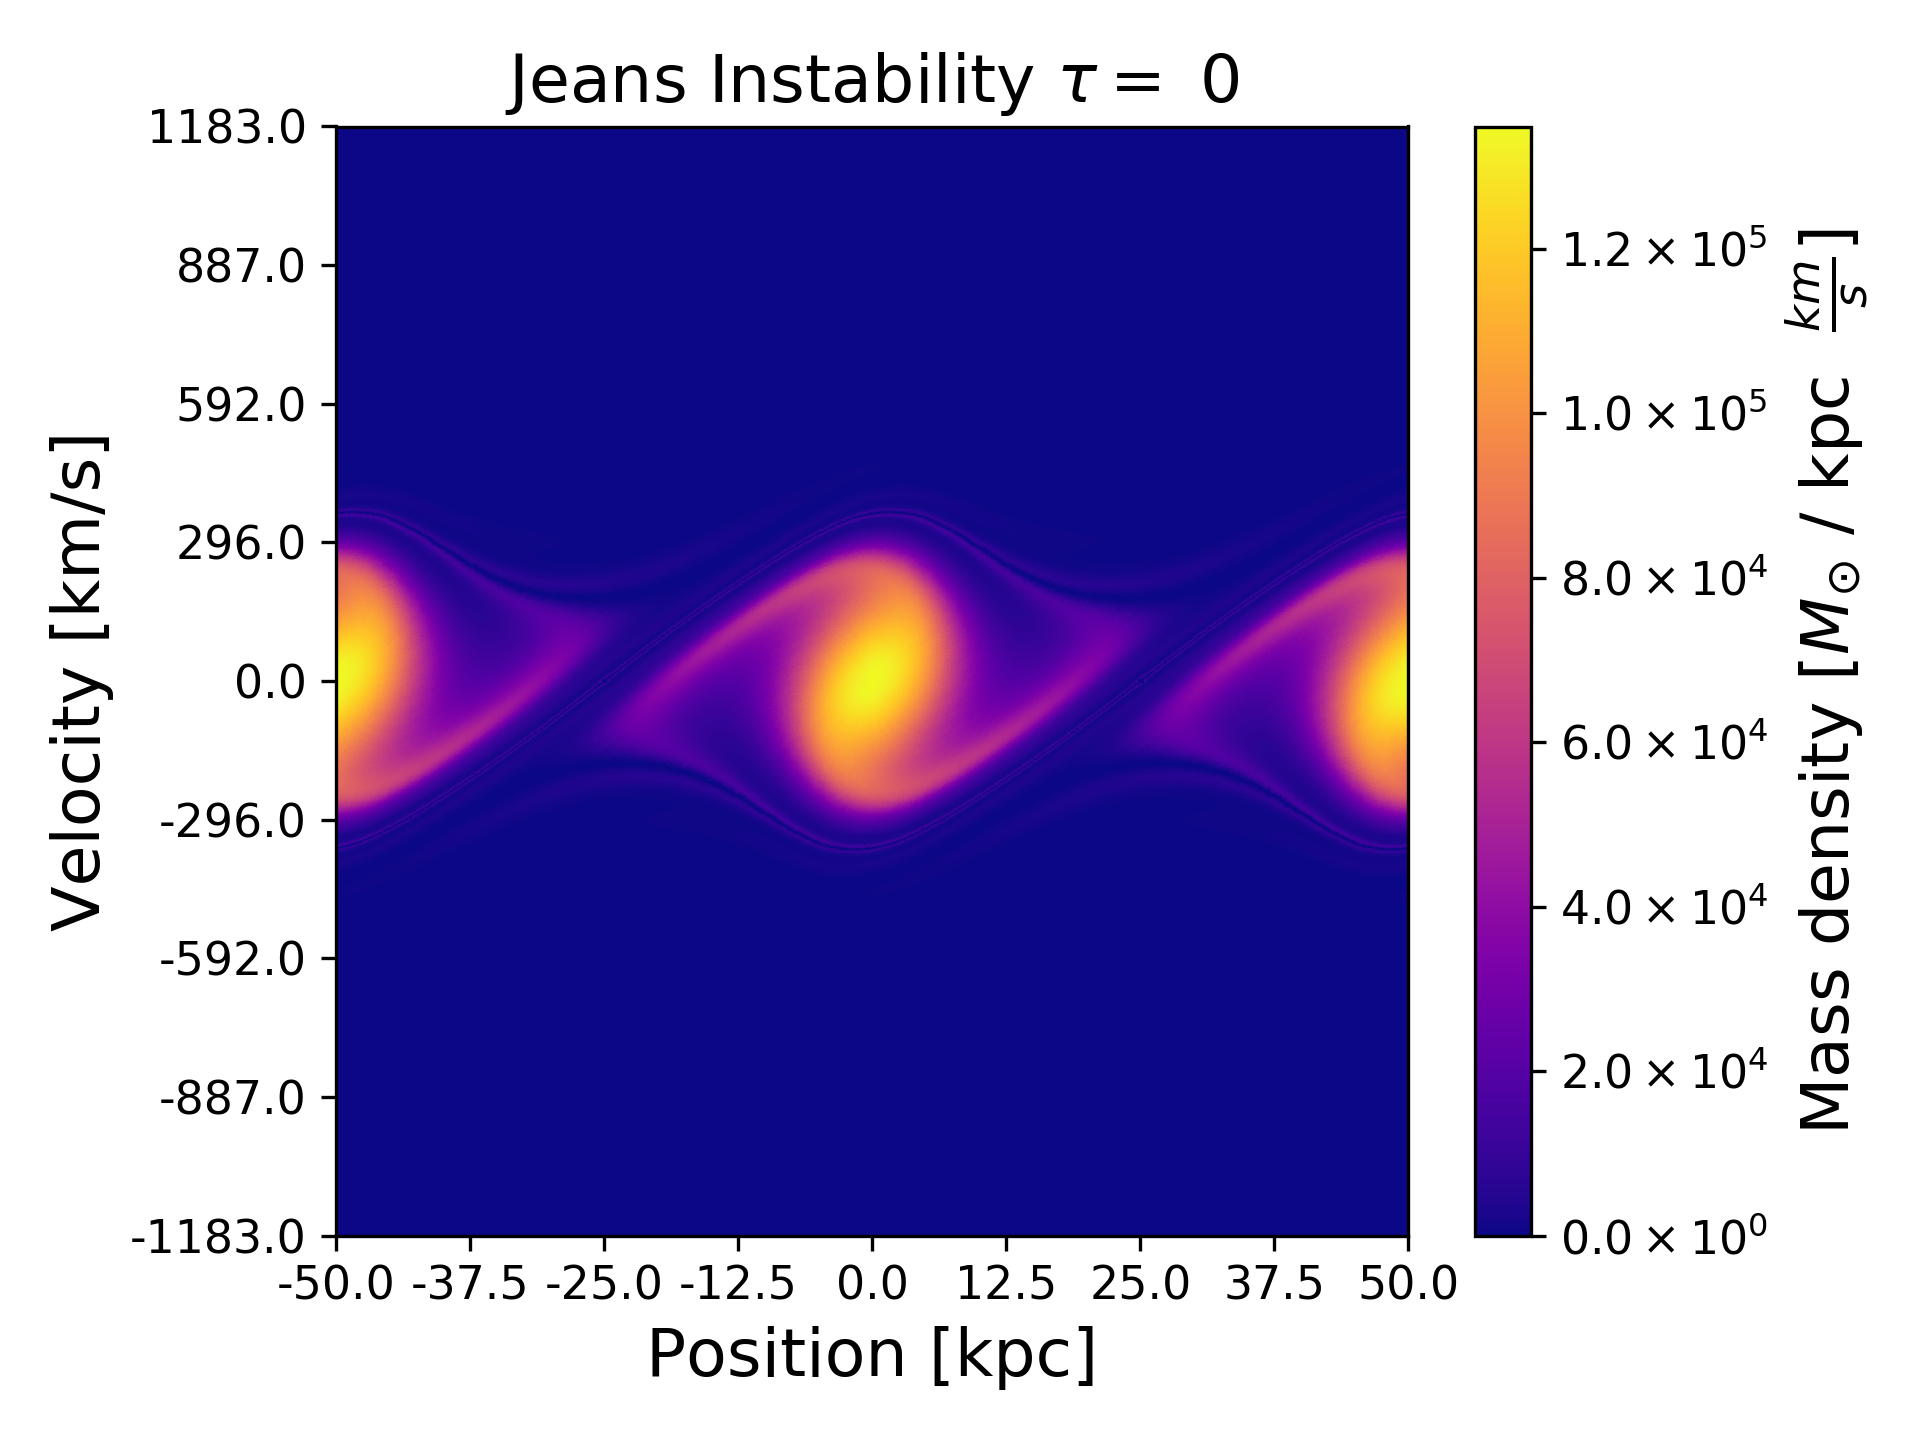
\includegraphics[scale=0.45]{imag/jeans22.png}
    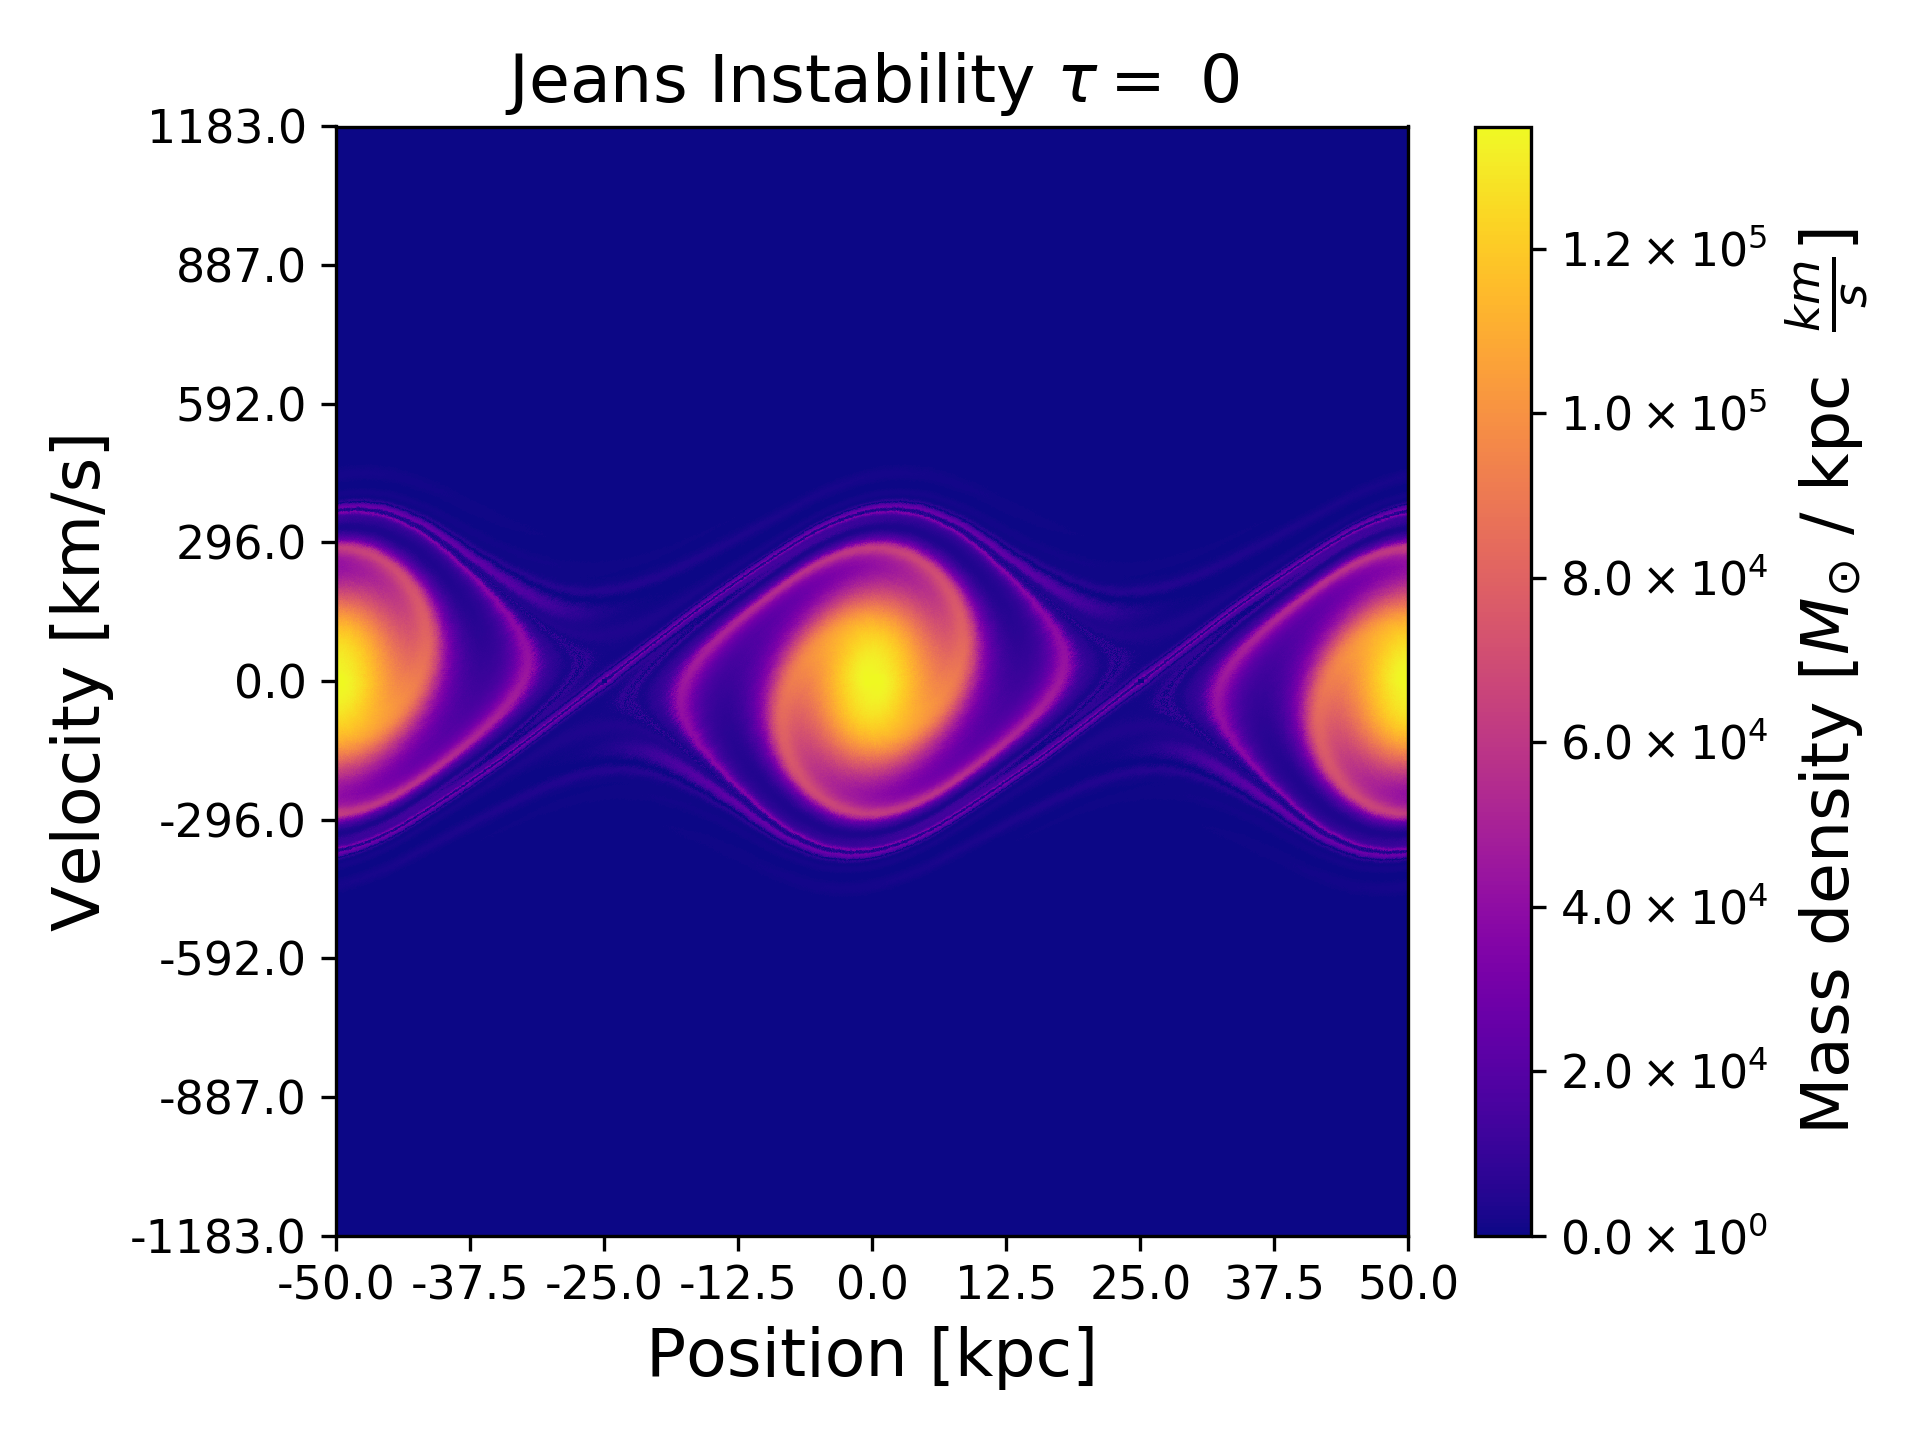
\includegraphics[scale=0.45]{imag/jeans40.png}
    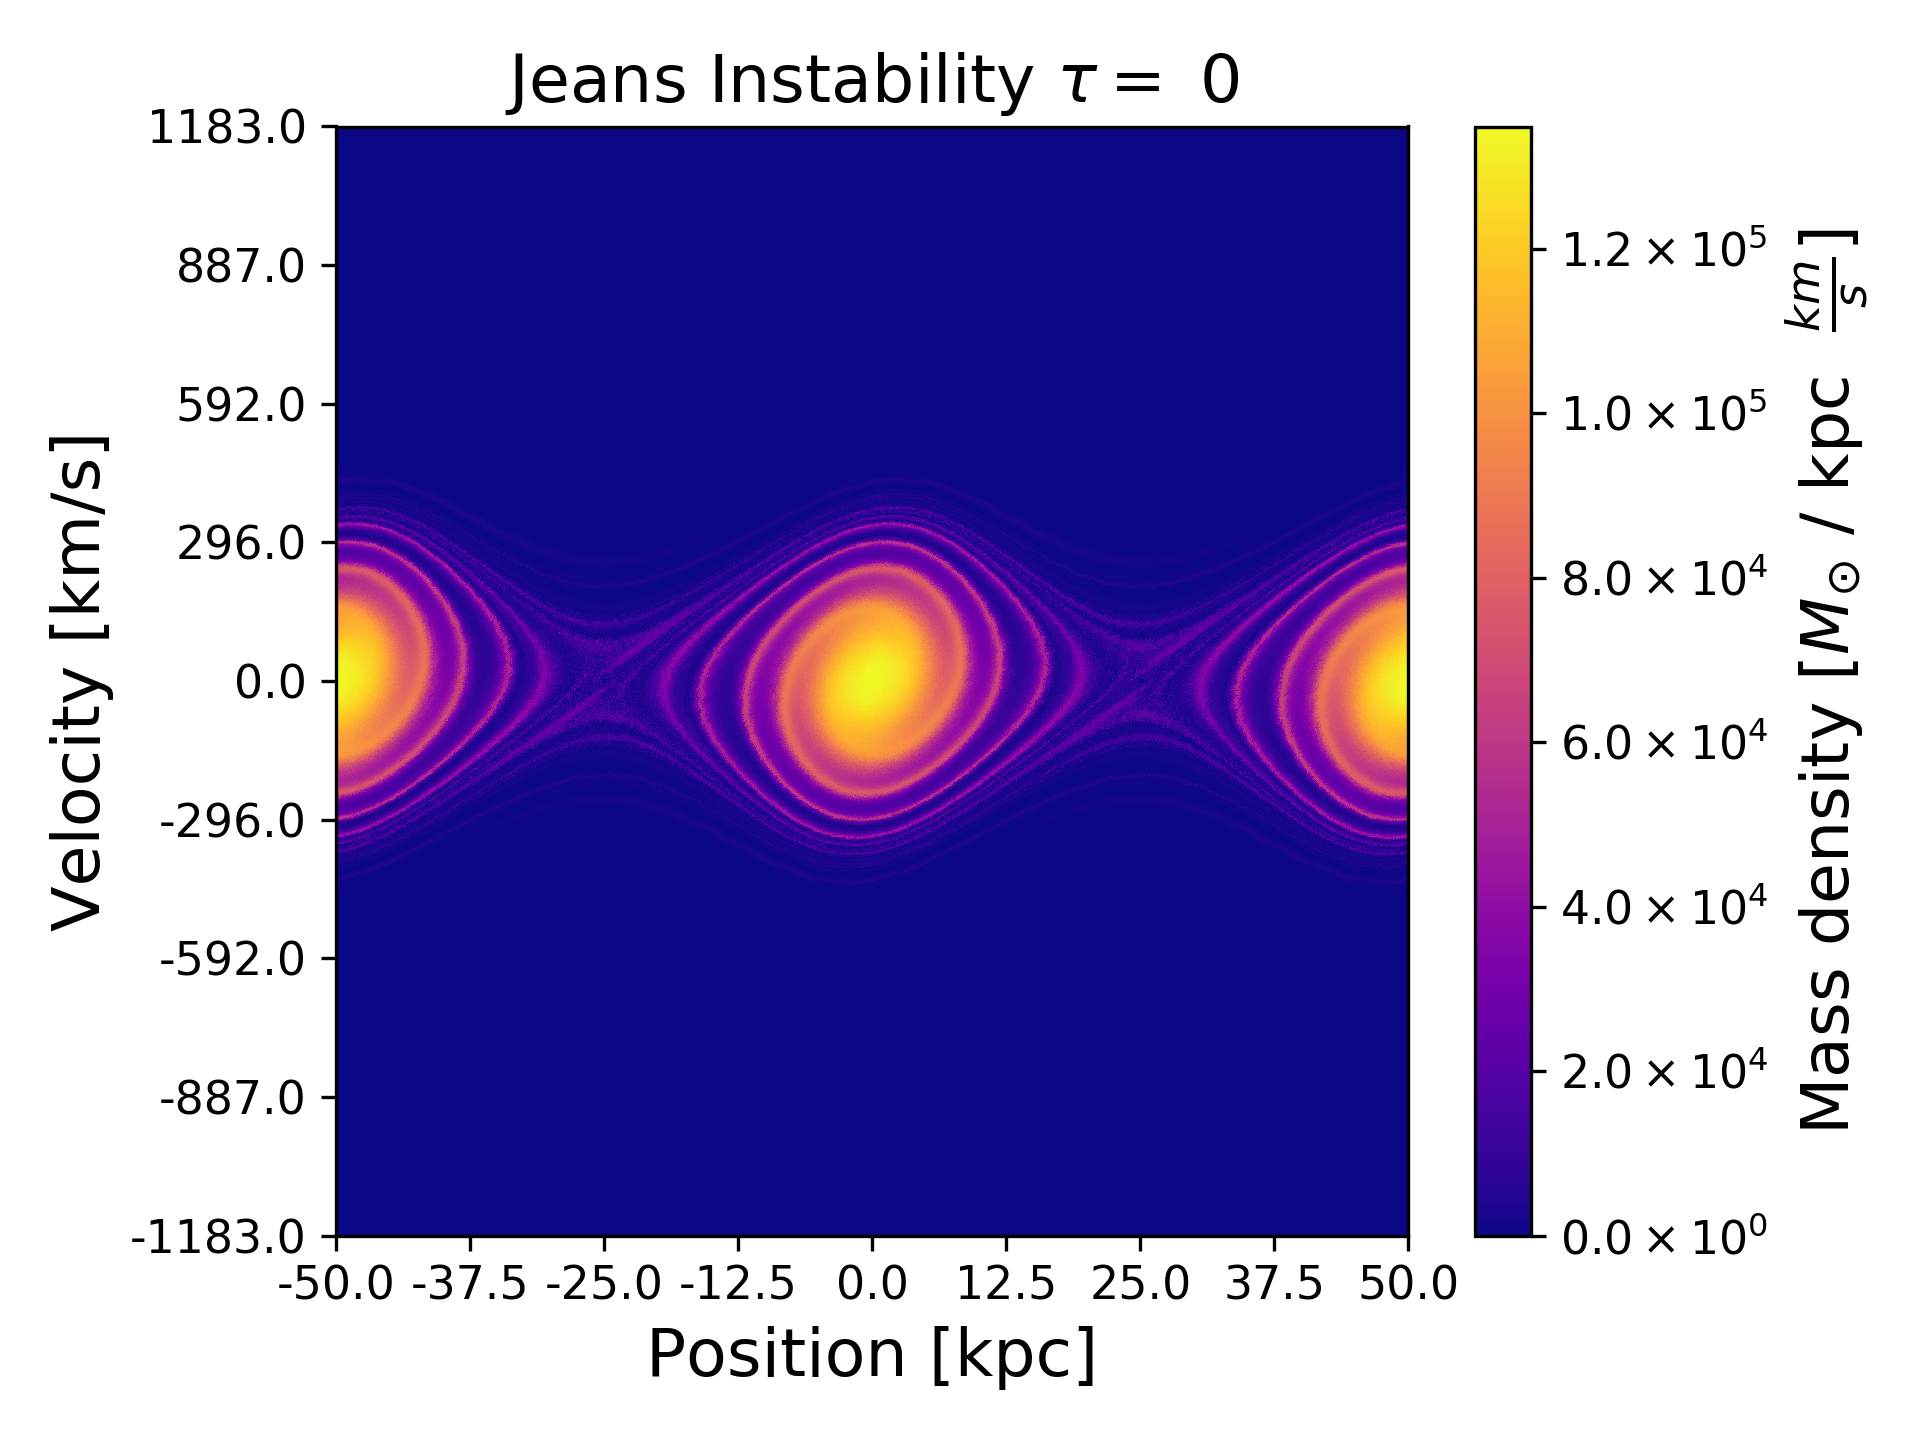
\includegraphics[scale=0.45]{imag/jeans90.png}
    \caption{Upper left: Phase space 72 million years after initialization. Upper right: Phase space 227 million years after initialization. Bottom left: Phase space 413 million years after initialization. Bottom right: Phase space 930 million years after initialization. The behavior is the same as three successive Gaussian conditions.}
    \label{1dJeans}
\end{figure}


The initial conditions are given by the function:
\begin{equation}
\f[0] = A_1\exp{-\frac{(x-0.4)^2}{2 \sigma_1^2} - \frac{v^2}{2 \sigma_v^2}} + A_2\exp{-\frac{(x+0.4)^2}{2 \sigma_2^2} - \frac{v^2}{2 \sigma_v^2}}
\end{equation}
Such that $A_i$ is a measure of the total mass of the ith halo, $\sigma_i^2$ is the variance of the Gaussian profile of the halo in the spatial axis, and $\sigma_v^2$ is the variance of the Gaussian profile in the velocity axis. The values used to initialize the simulation were:
\begin{align}
\sigma_1 &= 0.04 \ \text{us} \\
\sigma_2 &= 0.04  \ \text{us} \\
\sigma_v &= 0.06 \ \text{us} \\
A_1 &= 40 \ \text{um} \\
A_2 &= 30  \ \text{um}
\end{align}
Given the collisionless nature of this run, we expect the halos to simply pass through each other \emph{without any loss of energy} due to the collision. In other words, the \emph{density} profiles will have a periodic movement and will eventually return to their initial location.
In the phase space we see that each halo forms the clockwise spiral from the Gaussian initial conditions. In addition to that, we can see how when the halos occupy the same spatial position, they have very different velocities, which keeps them decoupled. The evolution of the phase space can be seen in figure \ref{phaseNoColBullet}. The oscillations in the spatial density can be seen in figure \ref{densNoColBullet}
\newpage
\begin{figure}[h!]
    \centering
    %\includegraphics[width=10cm,height =7cm]{Diapositiva1.jpg}
    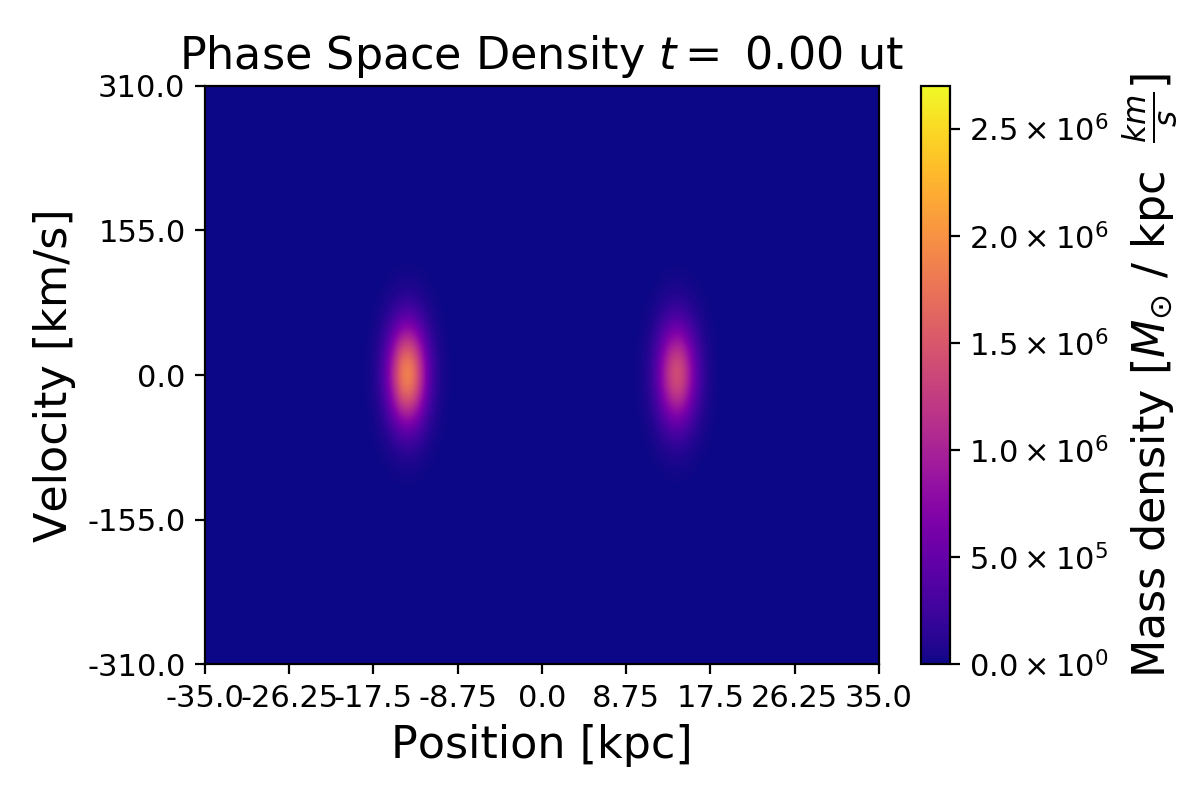
\includegraphics[scale=0.45]{imag/bullet0.png}
    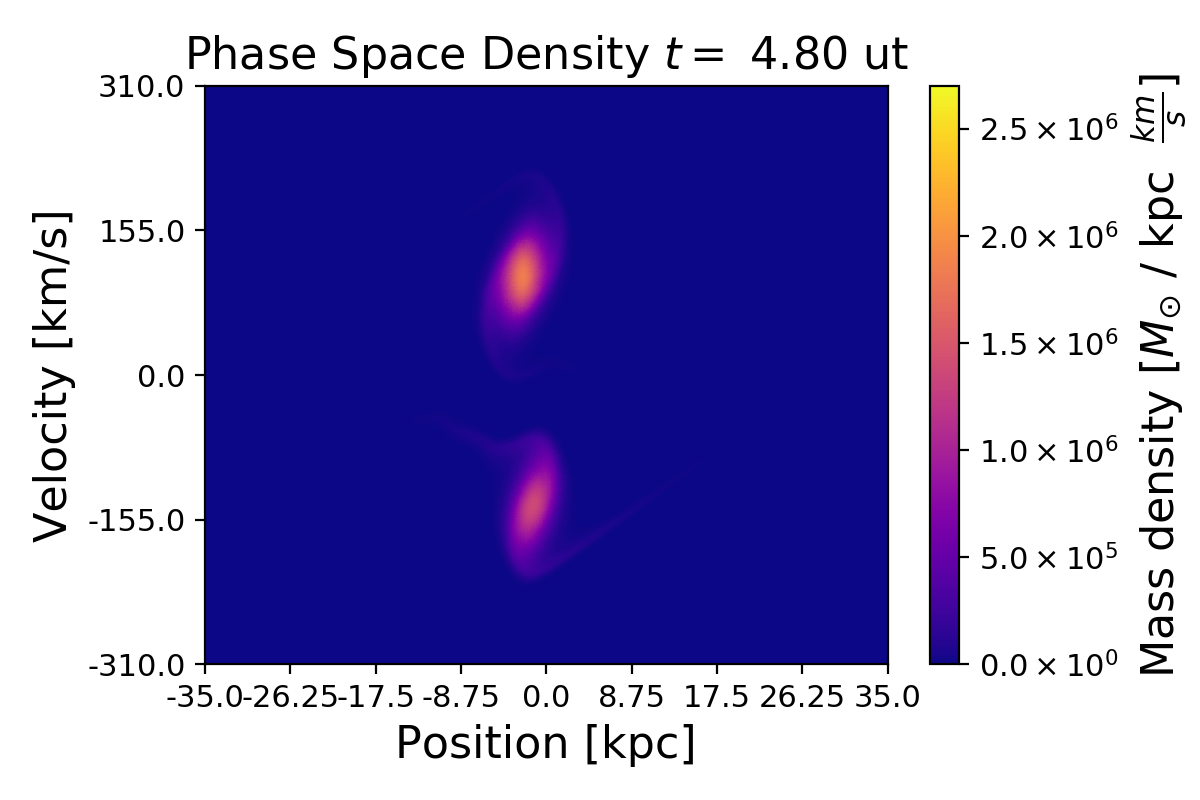
\includegraphics[scale=0.45]{imag/bullet12.png}
    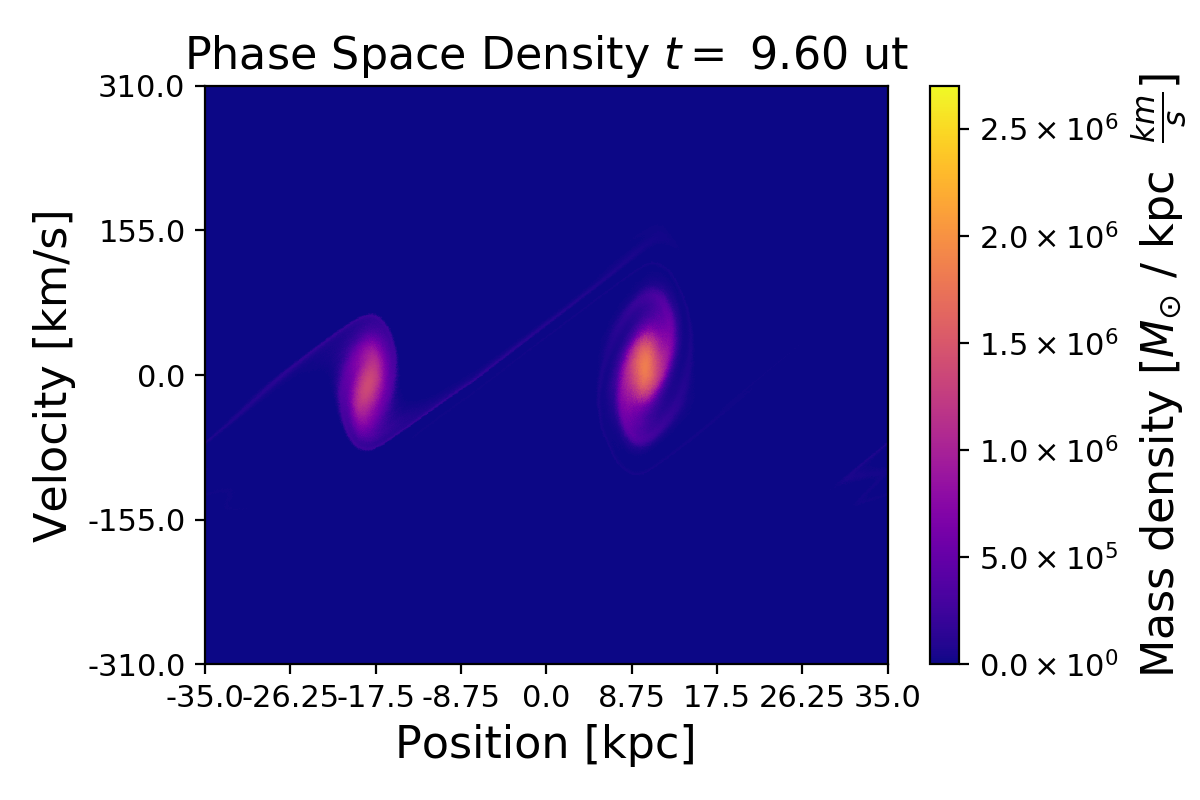
\includegraphics[scale=0.45]{imag/bullet24.png}
    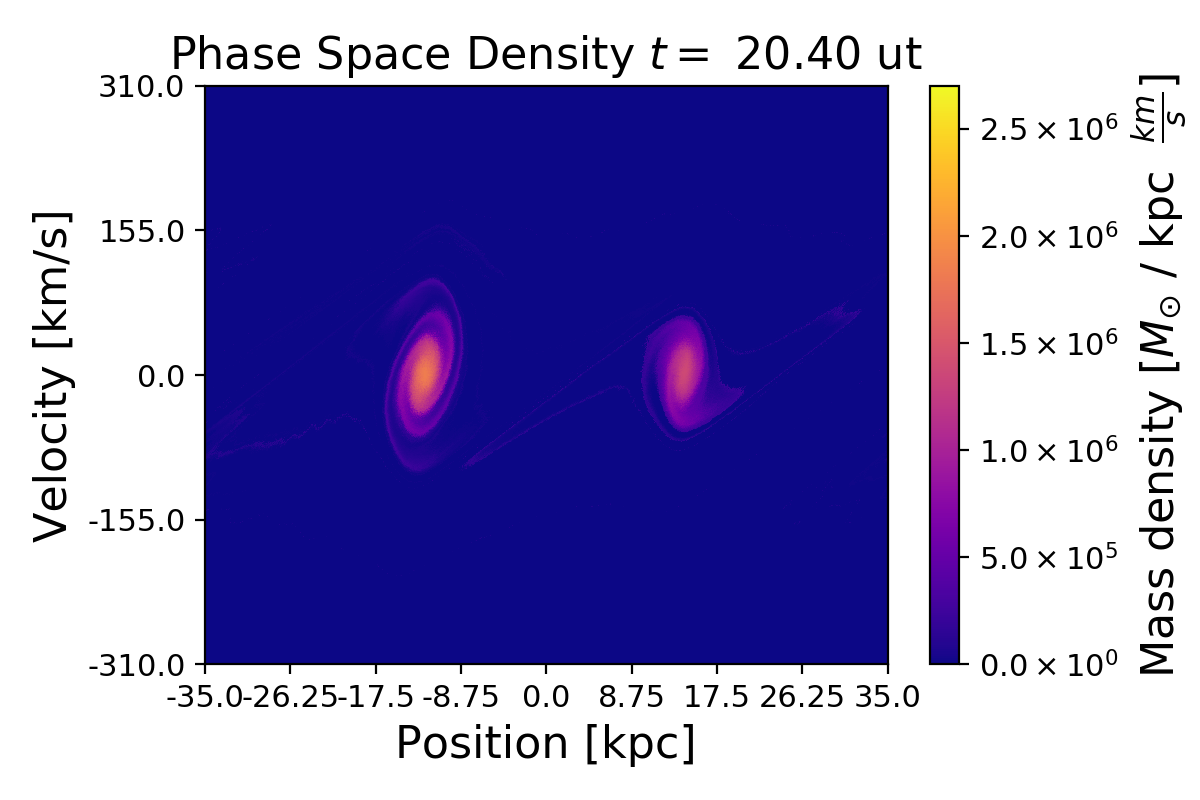
\includegraphics[scale=0.45]{imag/bullet51.png}
    \caption{Upper left: phase space initialization of the \emph{Bullet Cluster} run. The right halo is slightly less massive (dimmer). Upper right: phase space during the spatial collision of the halos. The gap in the velocity axis keeps the halos decoupled. Bottom left: phase space with the position of the halos switched regarding the centre of mass and the initial conditions. Bottom right: the system after a full period. The halos are at their initial position but their velocities have changed due to the evolution of each Gaussian.}
    \label{phaseNoColBullet}
\end{figure}

\begin{figure}[h!]
    \centering
    %\includegraphics[width=10cm,height =7cm]{Diapositiva1.jpg}
    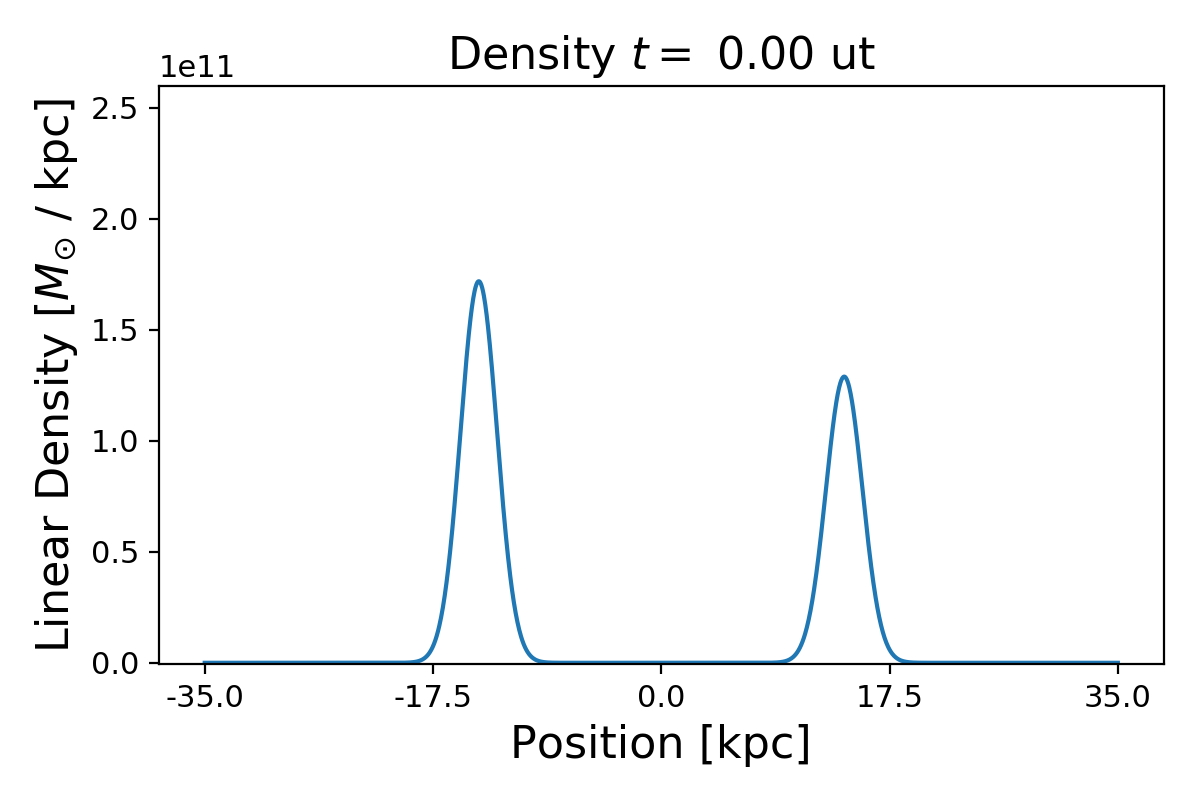
\includegraphics[scale=0.45]{imag/bulletD0.png}
    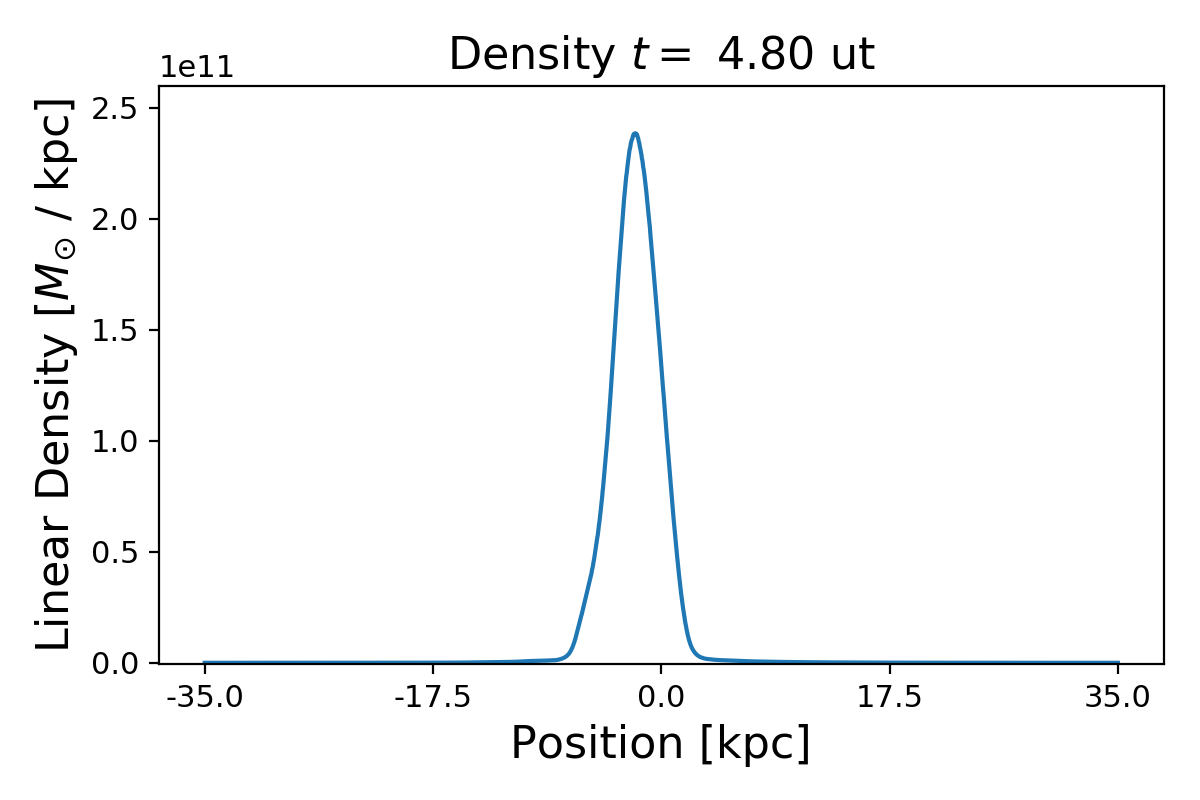
\includegraphics[scale=0.45]{imag/bulletD12.png}
    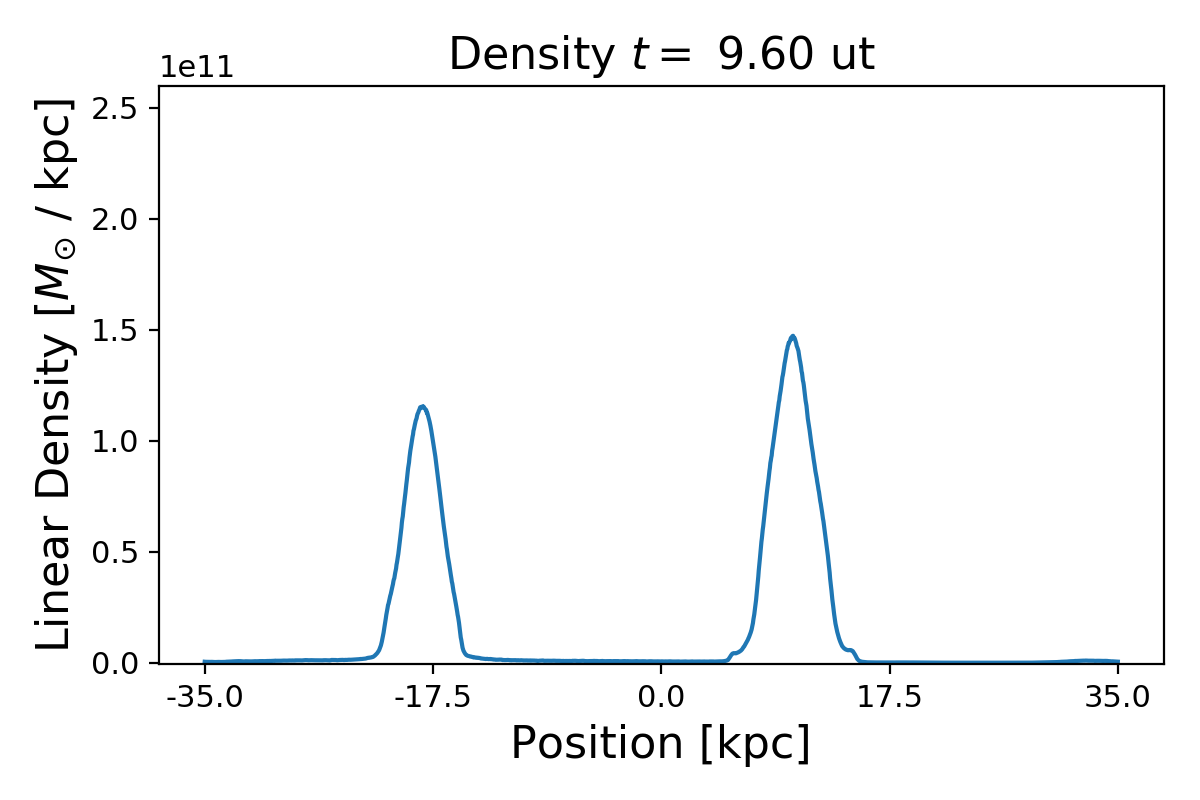
\includegraphics[scale=0.45]{imag/bulletD24.png}
    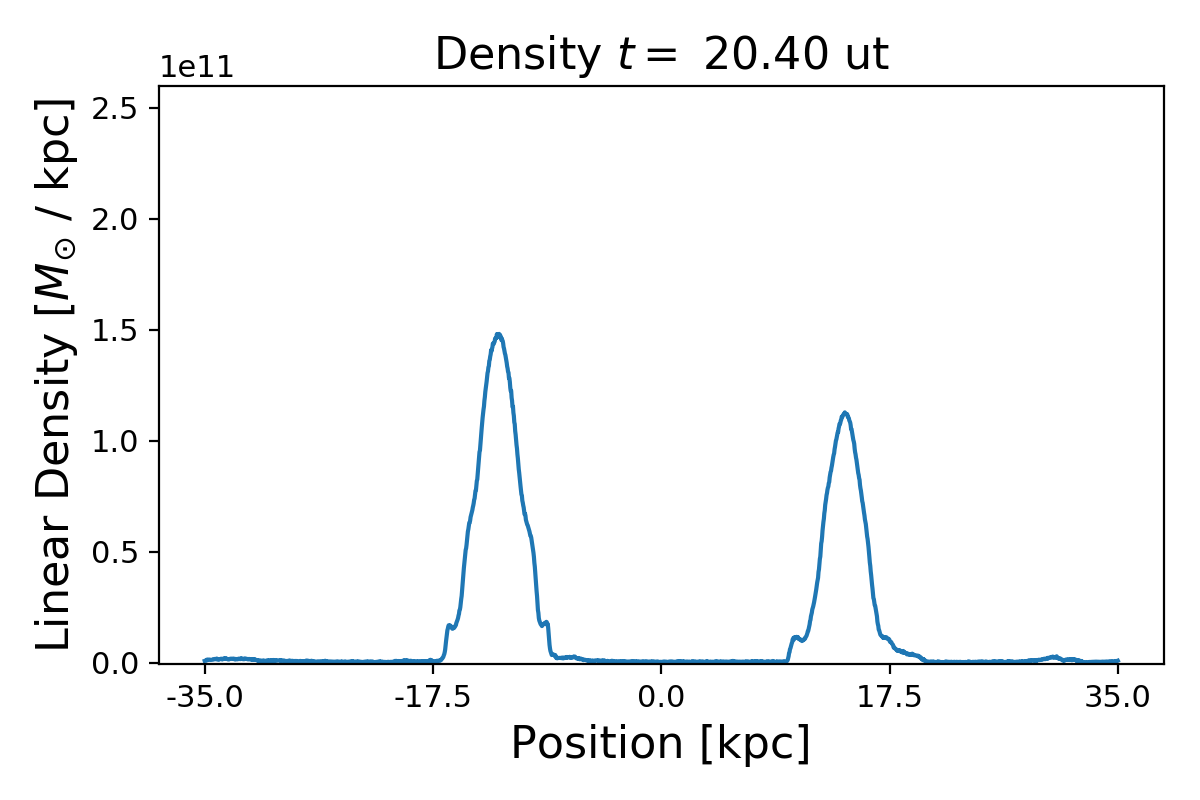
\includegraphics[scale=0.45]{imag/bulletD51.png}
    \caption{Upper left: density initialization of the \emph{Bullet Cluster} run. Notice that the left halo is heavier. Upper right: density during the spatial collision of the halos. Bottom left: density when the halos have switched position with regards to the centre of mass. Bottom right: the system after a full period. The halos are at their initial position but their velocities have changed.}
    \label{densNoColBullet}
\end{figure}


\newpage
\subsection{The collisional case}
Now, for the collisional case we are going to implement the Gaussian initial conditions as an introductory example, and then use the insight to interpret more easily the Bullet Cluster-like scenario.
Recalling the discussion on choosing a $\tau$ (see \ref{metodologiaBGK}), the final value was unit dependent. The value of $\tau$ in the units used in this section is $$\tau =8972 \ \text{ut}$$ Once again, we start with the Gaussian initial conditions.
We ran the simulation with exactly the same parameters as in the no collisional case and observed the evolution of the phase space.
The value of $\tau$ implies a very small collisional term.
Therefore, if we looked at the phase space distribution of the collisional case in the same way as we did in the last section, we would not be able to spot any difference between the two cases. Instead of plotting the phase space of the collisional case, we choose to plot the percentage difference between the cases: %TODO depronto haya que cambiar todos los porcentual a percentage 
\begin{equation}
\label{Zeta}
Z = 100\qty(\frac{f_{\tau}(\rv,t) - f_0(\rv,t)}{f_0(\rv,t)})
\end{equation}
With $Z$ being the percentual difference of the collisional case with the collisionless case. This representation will allow us to interpret more easily the effects of the collisional term in the distribution.

The evolution of the percentual difference in the phase space between the two cases can be seen in figure \ref{phaseColGauss}. In it we can appreciate  two main regions: a blue region (dominated by collisionless dark matter), and a red region (dominated by collisional dark matter). The collisionless fluid has higher velocities in the centre of the spatial distribution (the blue region), but the collisional distribution has a higher density in the tails of the Gaussian, implying a lower central density peak. This lower central peak in the spatial density can be observed directly in figure \ref{densColGauss}, where values higher than zero correspond to higher collisional density, and lower than zero to a higher collisionless density. Now it is easy to see that the collisional peak is about 20 percent lower than its collisionless counterpart and remains that way, even after a very long time. 


\begin{figure}[h!]
    \centering
    %\includegraphics[width=10cm,height =7cm]{Diapositiva1.jpg}
    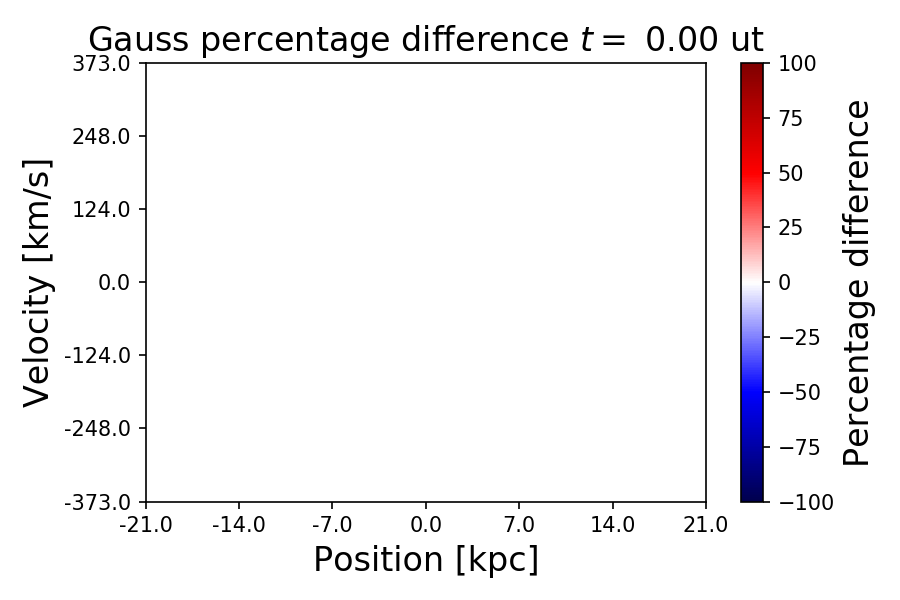
\includegraphics[scale=0.45]{imag/cGaussPhase0.png}
    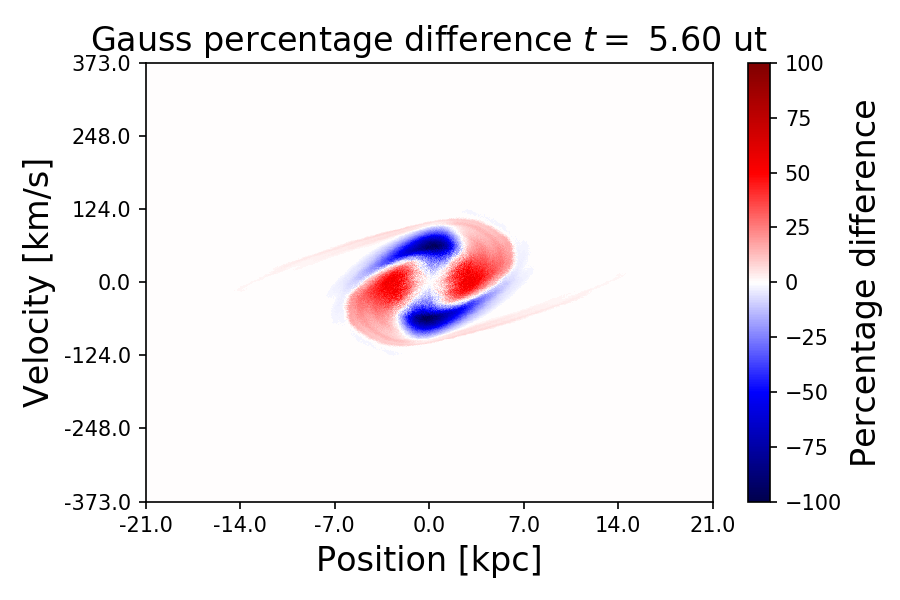
\includegraphics[scale=0.45]{imag/cGaussPhase14.png}
    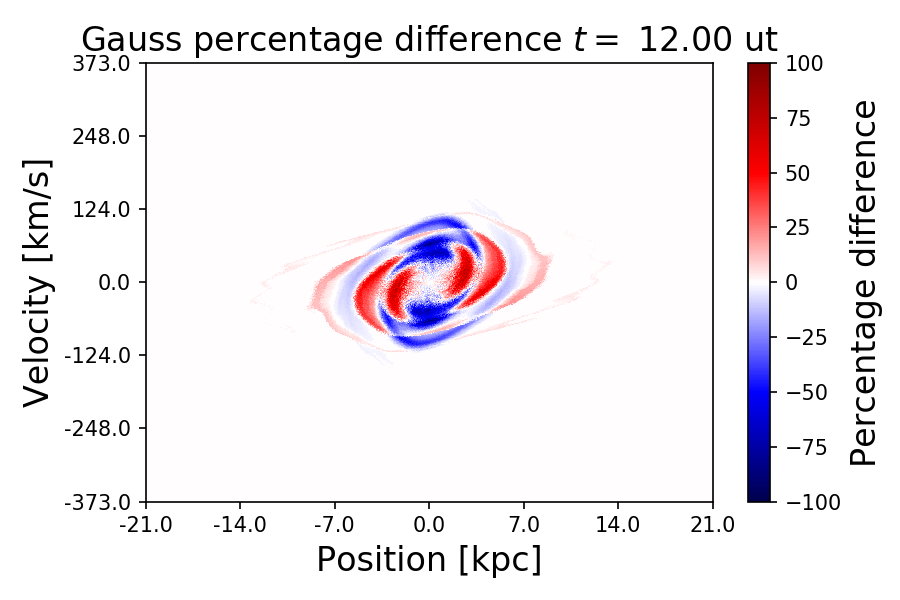
\includegraphics[scale=0.45]{imag/cGaussPhase30.png}
    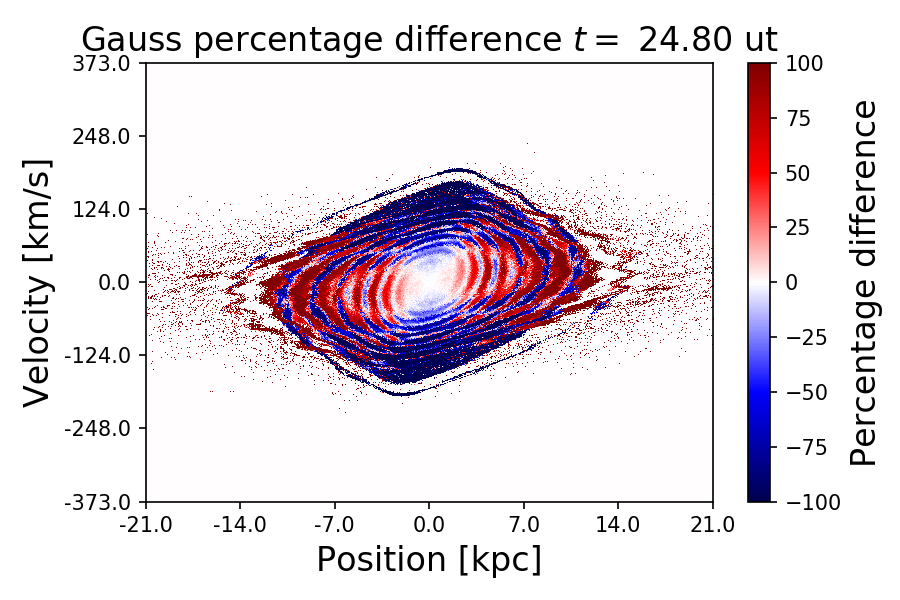
\includegraphics[scale=0.45]{imag/cGaussPhase62.png}
    \caption{Upper left: $Z$ at $t= 0$, we had exactly the same initial conditions in both cases. Upper right: $Z$ several timesteps after initialization. The collisional part has already a lower central peak and lower velocities in the centre. Bottom left: Eventually, the \emph{arms} of the distributions get out of sync but the general behavior remains. Bottom right: the distribution from the upper right image is now tainted by the arms. However, the general behavior is still the same, even after a long while.}
    \label{phaseColGauss}
\end{figure}

\begin{figure}[h!]
    \centering
    %\includegraphics[width=10cm,height =7cm]{Diapositiva1.jpg}
    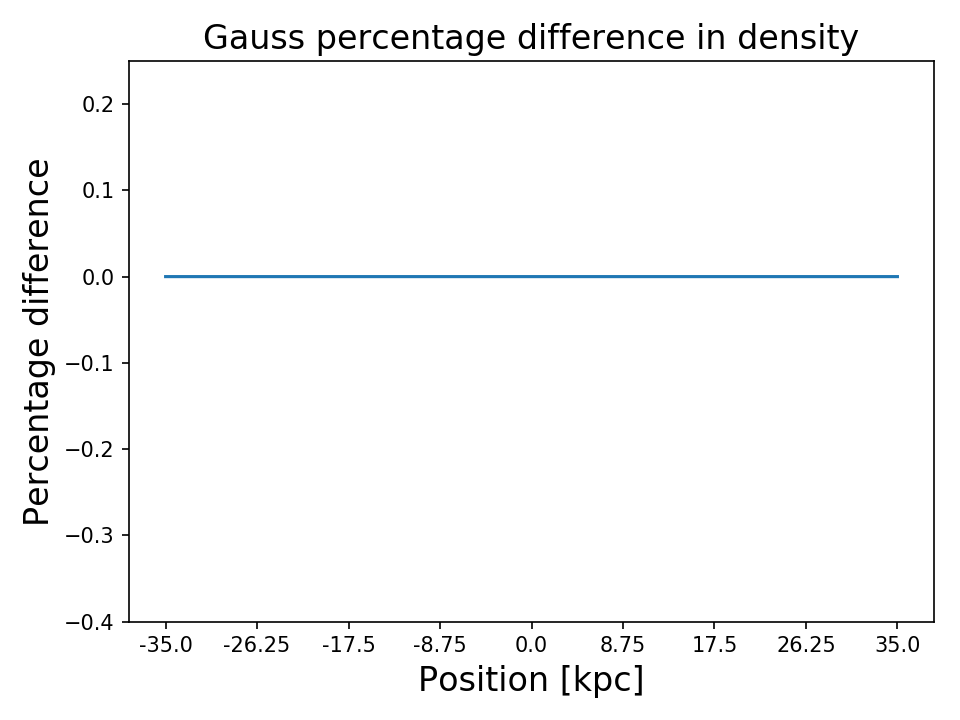
\includegraphics[scale=0.45]{imag/cGaussD0.png}
    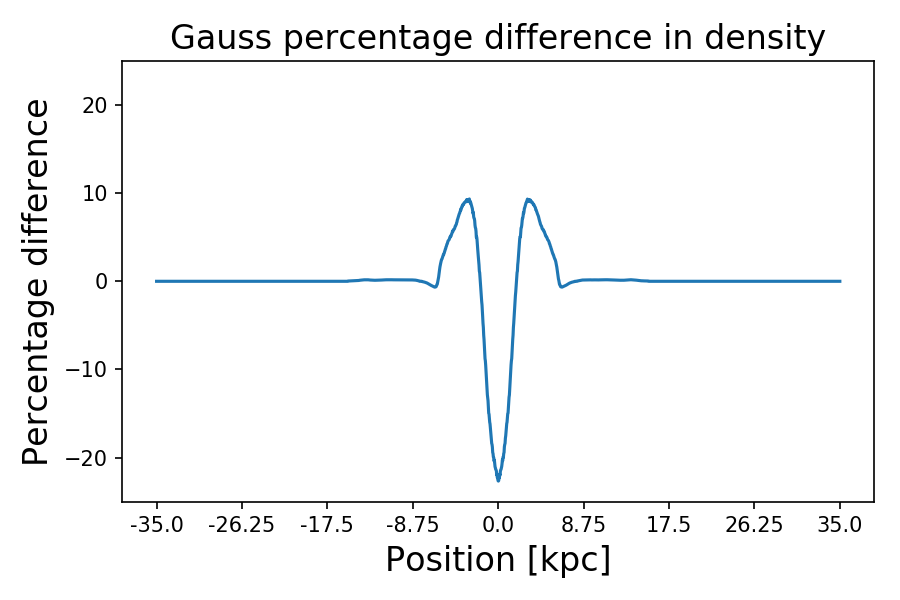
\includegraphics[scale=0.45]{imag/cGaussD14.png}
    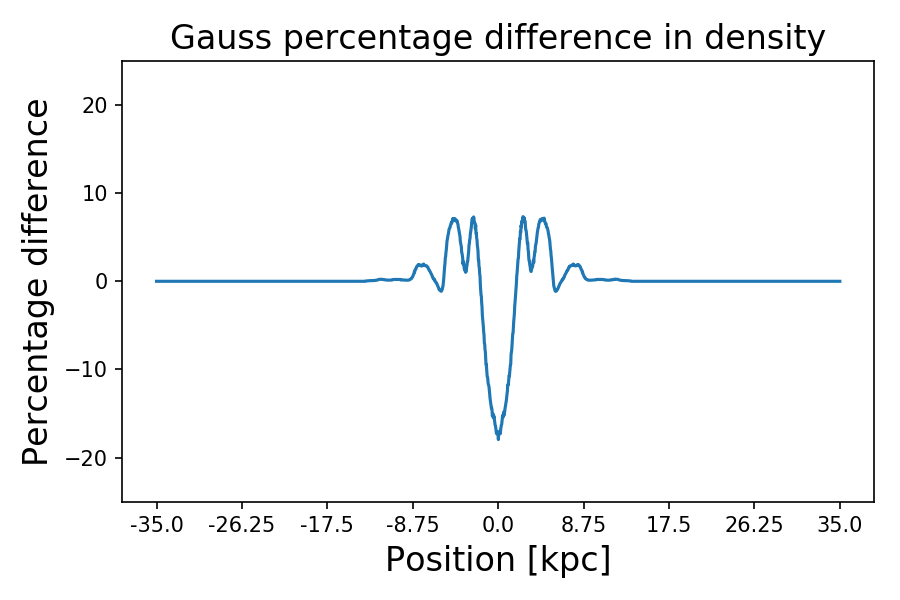
\includegraphics[scale=0.45]{imag/cGaussD30.png}
    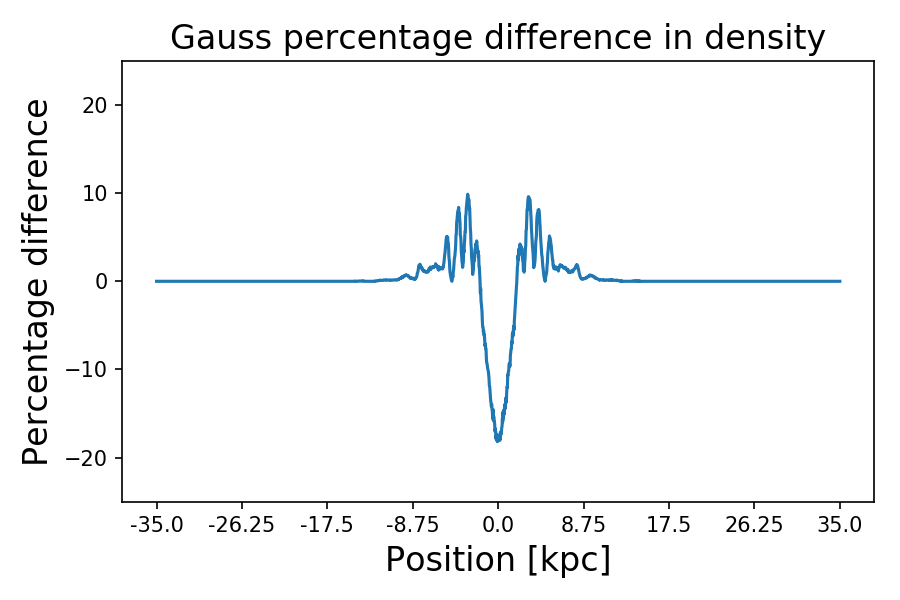
\includegraphics[scale=0.45]{imag/cGaussD62.png}
    \caption{Upper left: we initialize both cases with the same distribution. Upper right: after a while the collisionless case already dominates the central region and the collisional the tails. Bottom left: we observe small \emph{oscillations} in the tails but the general behavior remains. Bottom right: after a long while, the tails have some oscillations, nonetheless, the general behavior still remains. The oscillations correspond phase between the little bumps mentioned in the collisionless Gaussian case. Every density frame corresponds to the same frame in figure \ref{phaseColGauss}.}
    \label{densColGauss}
\end{figure}

Recapitulating, due to the collisional term we have two main effects:
\begin{itemize}
\item There is a considerable reduction of velocity in the central part of the spatial distribution.
\item There is a reduction of about 20$\%$ in the height of the central peak. Additionally, the regions outside the central peak have a higher velocity than their no collisional counterparts.
\end{itemize}

Now that we have introduced the collisional effects with the Gaussian example, we can proceed to the real case of interest: the Bullet Cluster. 

Recalling from \ref{bulletExplain}, Galaxy Clusters have three main components: a highly collisional baryonic gas, a collisionless distribution of galaxies, and a slightly collisional dark matter halo. Here, we simulated the slightly collisional dark matter component and compare it with the collisionless case.% In addition to that, we are also going qualitatively the hot baryonic gas as a very collisional fluid. %TODO si queda tiempo hacer un apéndice con TAU = 50

For this run we use the same simulation parameters as those of the no collisional case.
In the collisionless run the halos had a periodic movement, that was because there was no dissipation of energy.
Now that we include short range interactions, there is a loss of energy every time the halos collide (in addition to the loss of energy due to the internal evolution of each collisional Gaussian halo), and because of that, the halos will not return to their initial state. How long will it take for the halos to permanently merge is directly related to the relaxation time. Our relaxation time (8972 ut) is quite high, which is why we expect them to merge only after several collisions.

In figure \ref{phaseColBullet} we plot the phase space during the aphelion of the halos, expecting the distance between them to become smaller as time passes by. It is easy to appreciate that the system is permanently loosing energy and is{ bound to collapse.
After six collisions, the smaller halo becomes a current in the bigger one forming a single final halo.
This is a very different behavior from the collisionless case, in which the halos could oscillate forever.
In figure \ref{densColBullet} we plot the spatial density at the same time instants as in figure \ref{phaseColBullet}. It is clear that the halos are getting closer and will eventually merge. Notice that in the final frame, even though the halos have merged, the smaller halo is mostly around the heavier one and will fall inwards given enough time.

\begin{figure}[h!]
    \centering
    %\includegraphics[width=10cm,height =7cm]{Diapositiva1.jpg}
    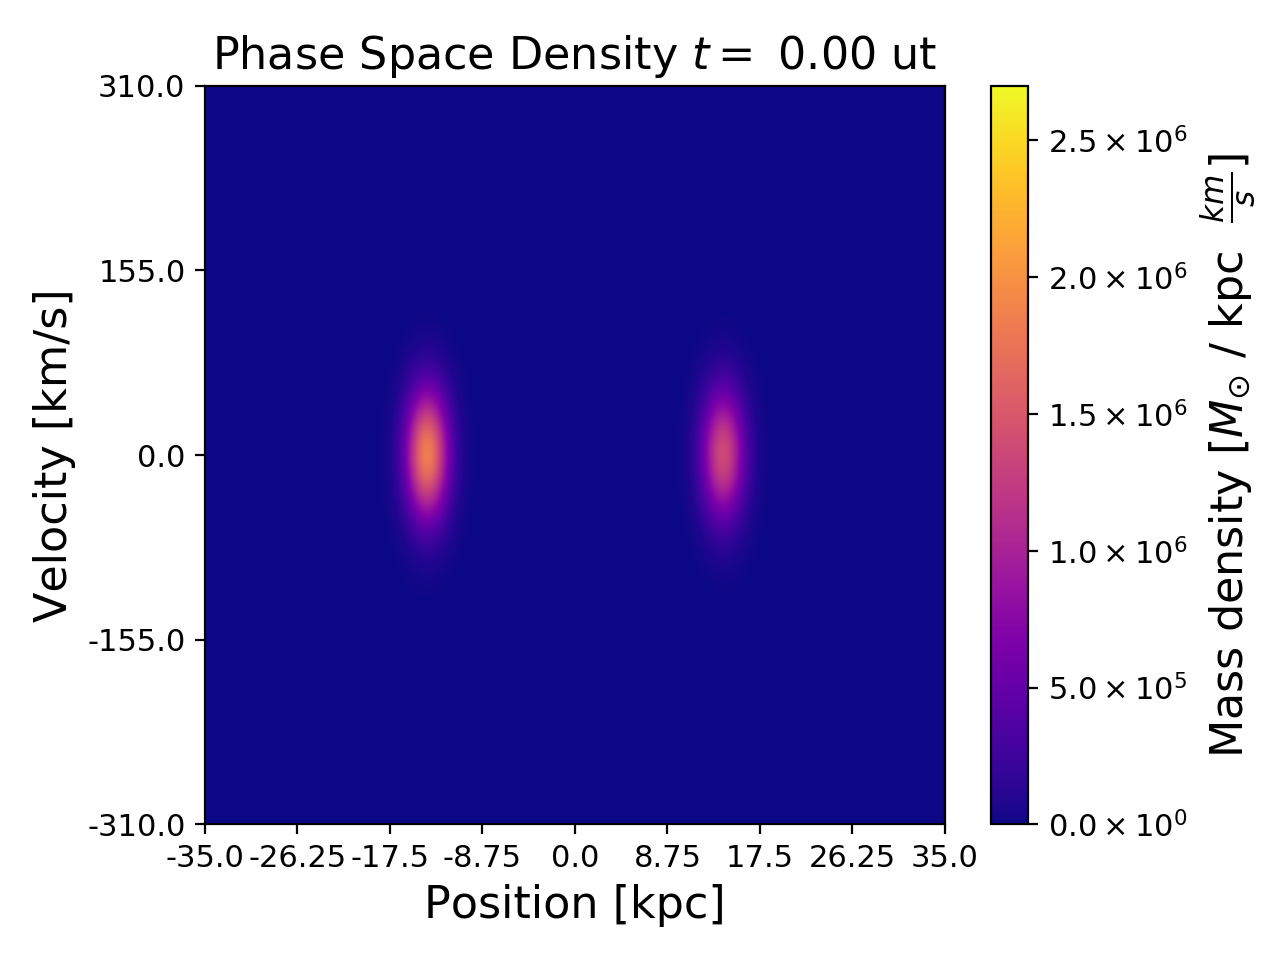
\includegraphics[scale=0.45]{imag/cBulletPhase0.png}
    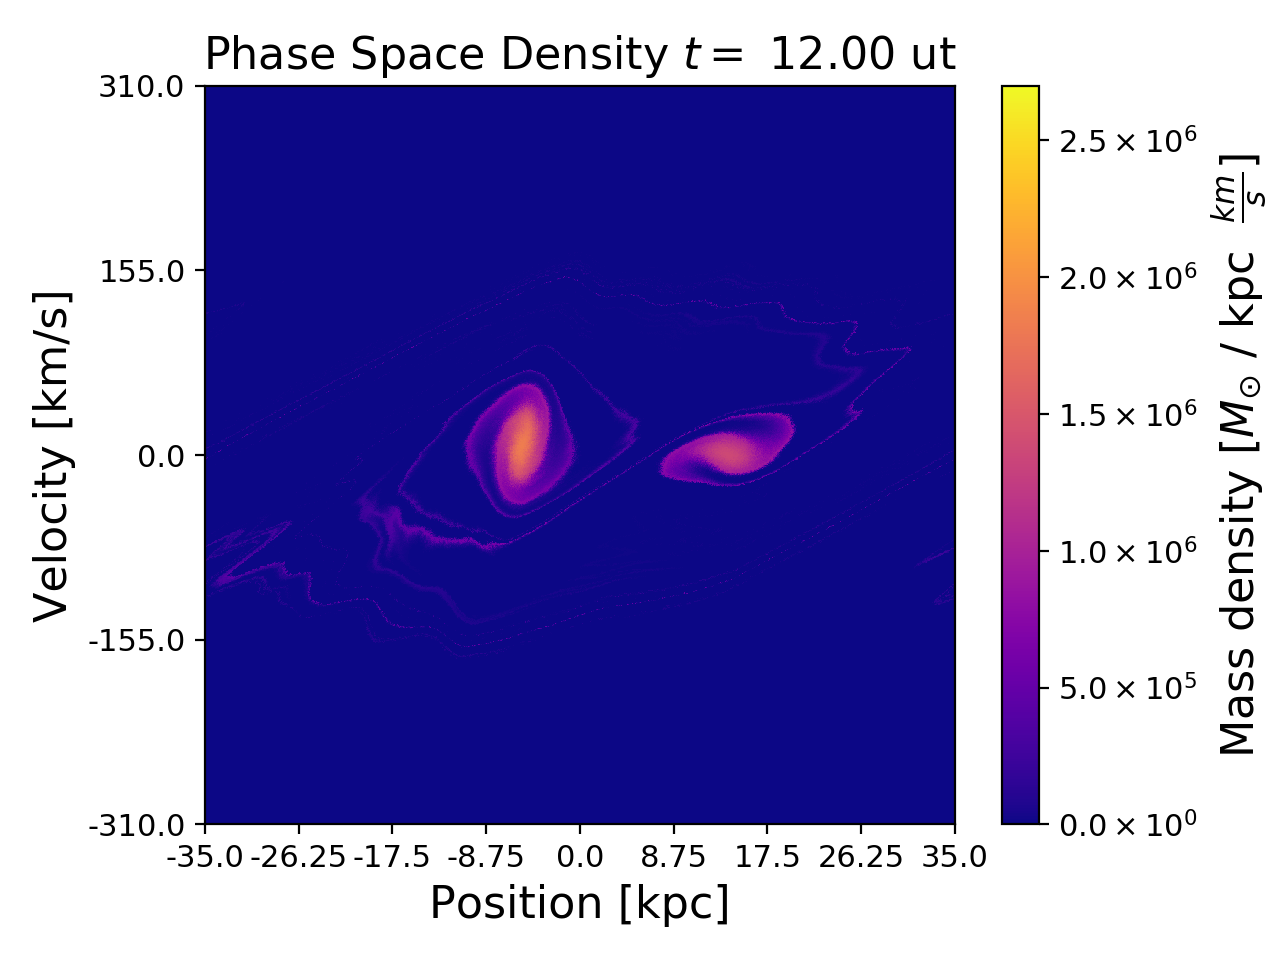
\includegraphics[scale=0.45]{imag/cBulletPhase30.png}
    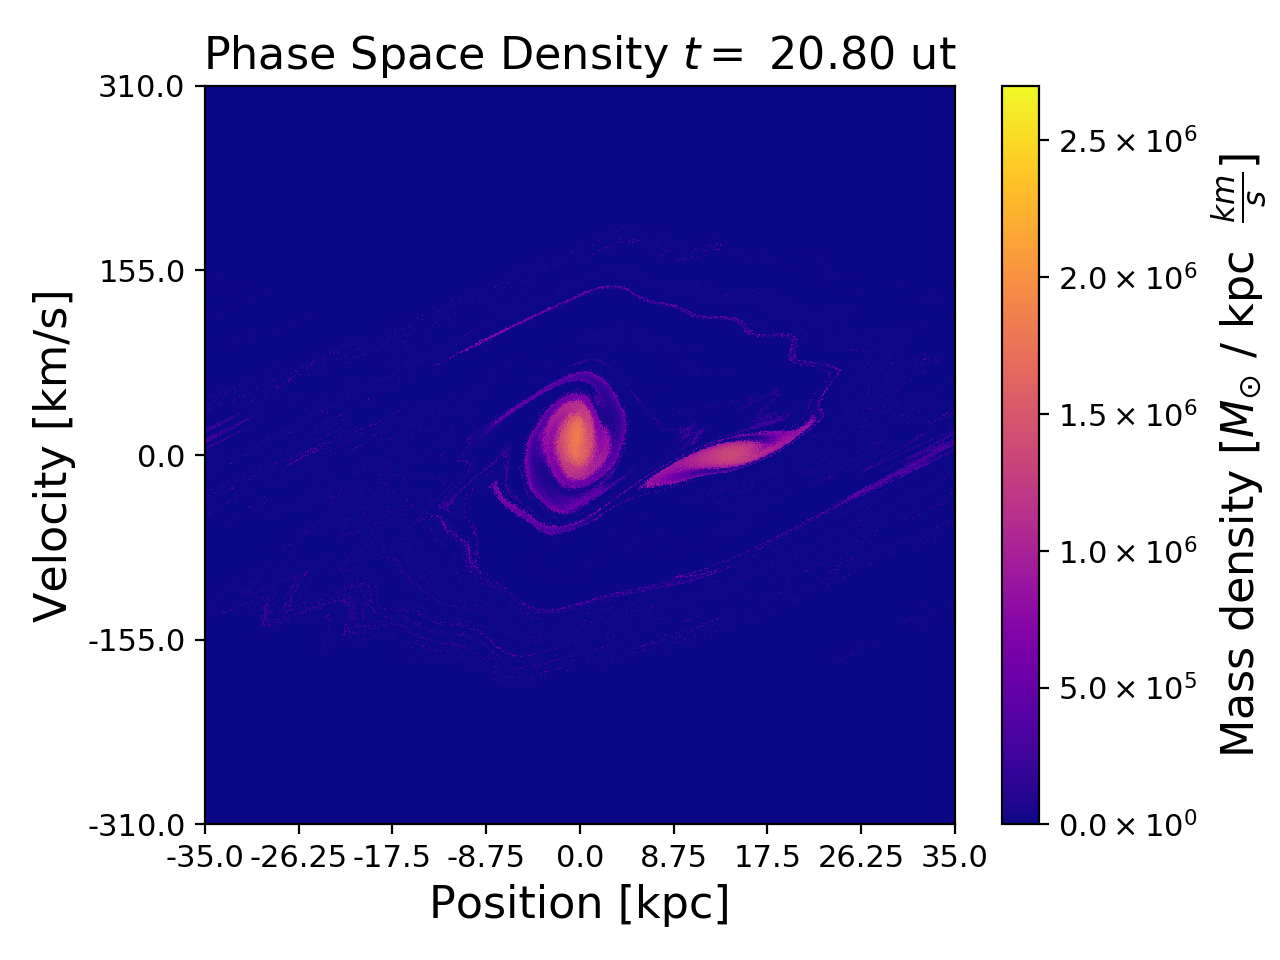
\includegraphics[scale=0.45]{imag/cBulletPhase52.png}
    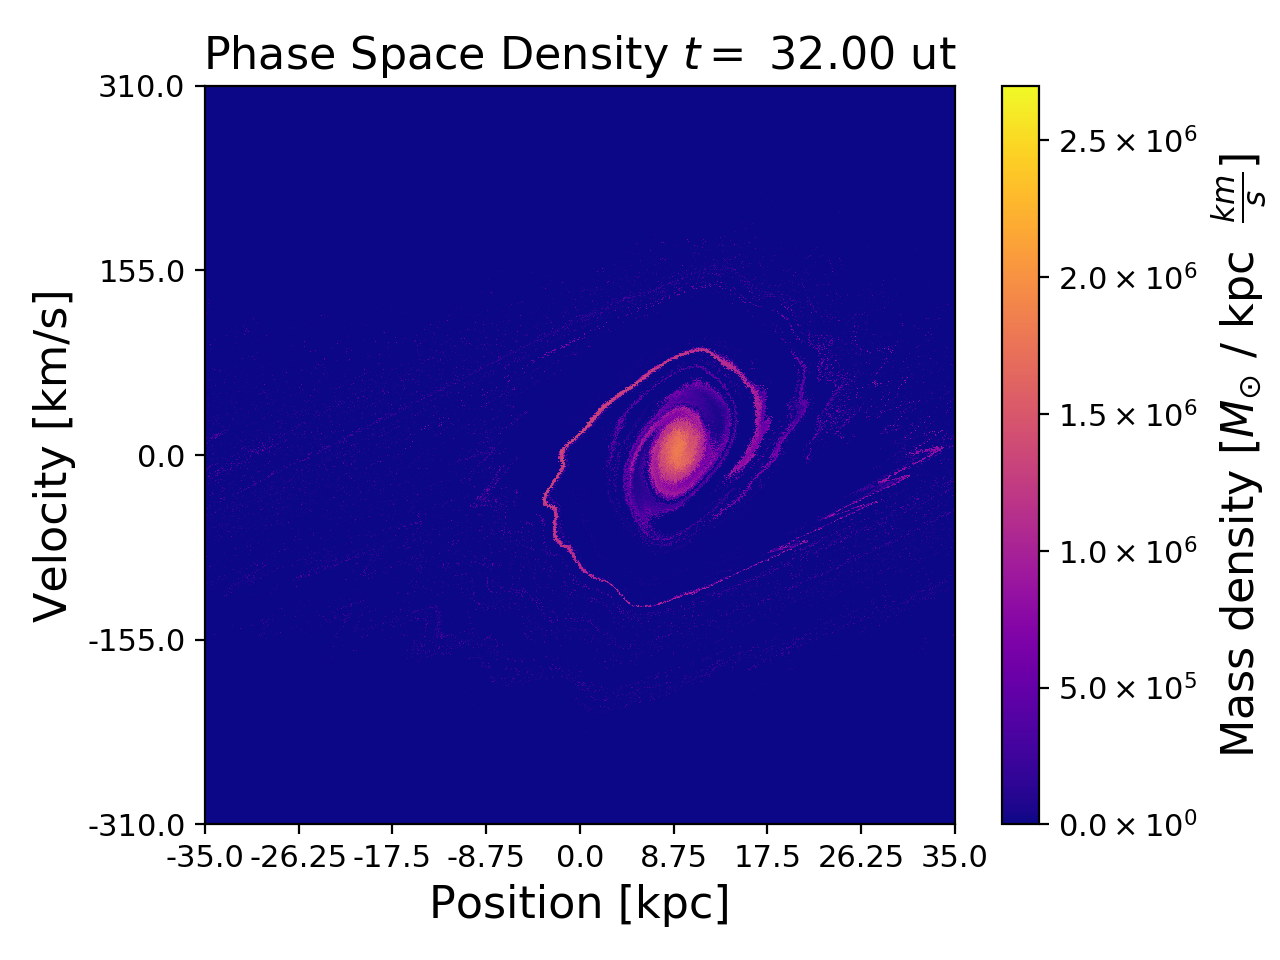
\includegraphics[scale=0.45]{imag/cBulletPhase80.png}
    \caption{Upper left: initial conditions for the phase space of the collisional Bullet Cluster scenario. Upper right: the phase space during the second aphelion since initialization. Note that the halos are closer together now as they have collided twice.  Bottom left: the phase space at the fourth aphelion since initialization, the halos have collided four times. The smaller halo is already collapsing towards the bigger one. Bottom right: the smaller halo has already collapsed into a current of  the bigger halo.}
    \label{phaseColBullet}
\end{figure}

\begin{figure}[h!]
    \centering
    %\includegraphics[width=10cm,height =7cm]{Diapositiva1.jpg}
    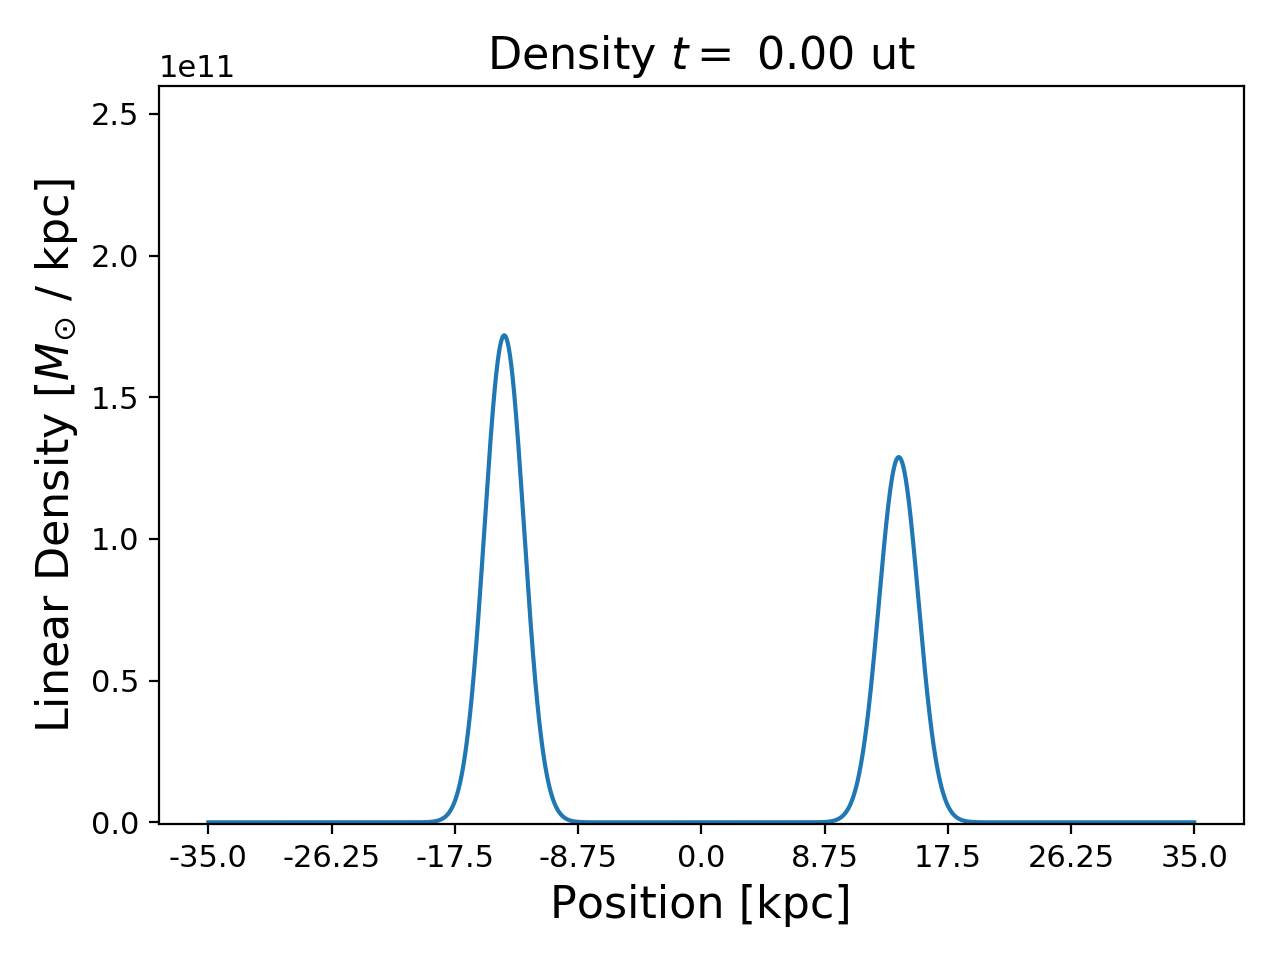
\includegraphics[scale=0.45]{imag/cBulletD0.png}
    \includegraphics[scale=0.45]{imag/cBulletD30.png}
    \includegraphics[scale=0.45]{imag/cBulletD52.png}
    \includegraphics[scale=0.45]{imag/cBulletD80.png}
    \caption{The spatial densities correspondent to the frames of figure \ref{phaseColBullet}. Upper left: initial conditions. Upper right: density during the second aphelion. We observe that there are more bumps than in the collisionless case and the Gaussians are closer. Bottom left: spatial density during the fourth aphelion. The distributions are now even closer, and the smaller Gaussian is starting to be absorbed by the bigger Gaussian. Bottom right: the spatial density at what would have been the sixth aphelion. The halos have merged now, but there are still some oscillations on the tails of the remainder distribution.}
    \label{densColBullet}
\end{figure}

\newpage
%TODO quitar el new page si es necesario

Finally, we close the two dimensional results comparing the phase space evolution of the collisional case with its no collisional counterpart.
We plot the percentage difference $Z$ as defined for the Gaussian case in figure \ref{colBulletPhase}.
The first frame shows the distributions at their first aphelion, here the two distributions are not too different but the halos of the collisional case are closer together.
In the second frame we observe the collisional distribution on its second aphelion, but the collisionless distribution (blue) has barely moved. The third frame is during the second aphelion of the no collisional distribution, and shows that the collisional halos are already collapsing into one heavier halo.
The last frame shows the fourth aphelion of the no collisional case, here, the smaller halo of the collisional distribution has collapsed into a current in the bigger halo.


\begin{figure}[h!]
    \centering
    %\includegraphics[width=10cm,height =7cm]{Diapositiva1.jpg}
    \includegraphics[scale=0.45]{imag/diffBullet20.png}
    \includegraphics[scale=0.45]{imag/diffBullet28.png}
    \includegraphics[scale=0.45]{imag/diffBullet50.png}
    \includegraphics[scale=0.45]{imag/diffBullet94.png}
    \caption{Upper left: percentage difference at half the period of the collisionless case. Here they have collided once. Upper right: the collisional distribution has completed one oscillation, meanwhile, the collisionless fluid has barely moved since last frame. Bottom left: the collisionless distribution has completed a period. The collisional smallest halo is already collapsing into a current of the heavier halo. Bottom right: the collisionless distribution has once again completed a period (has collided four times in total). The smallest collisional distribution has been completely tore apart by the heaviest and is now just a current in the outskirts of the final distribution }
        \label{colBulletPhase}
\end{figure}
%TODO arreglar aphelio.
%Now, for the hot baryonic gas we choose a relaxation time that mirrors its highly collisional nature. 
%This relaxation time is not linked to any particular investigation, as it only serves our interest of testing the simulation when the fluid is highly collisional (highly in astrophysical standards). The relaxation time chosen is $$\tau = 50 \ \text{ut}$$

%This time we plot both the collisional phase space, and the percentage difference. Given our rather low relaxation time, we expect the distribution to lost a considerable amount of energy each collision. The system quickly collapses into one agglomeration of mass. 


\newpage
\section{Four dimensional phase space}
In the case of the four dimensional phase space we need four axes to describe the phase space. Increasing the number of axes in regards to the two dimensional case means that we are going to have to sacrifice a lot of resolution in order to comply to RAM memory constrains. The four dimensional grid used is characterized by:
\begin{align}
W_{min} &= -1\\
W_{max} &= 1\\
N_w &= 128\\
dw &= 1/64
\end{align}
Likewise, the units to use are:
\begin{align}
1\ us &= 50\ \text{kpc}\\
1\ ut &= 0.003 \ \text{t}_0\\
1\ um &= 10^{11} \ \text{M}_{\astrosun}
\end{align}
With t$_0$ being the age of the universe today, \text{M}$_{\astrosun}$ being a solar mass and a kiloparsec (kpc) is equal to $3.0857\e{19}$ m. In this units, the gravitational constant has a value of:
\begin{equation}
G = 0.006141 \ (1 \ us)^3 \ (1 \ um)^{-1} \ (1 \ ut)^{-2}
\end{equation}
\subsection{No collisional case}
The four dimensional case is initialized using a Gaussian distribution. The main interest in the Gaussian case is to test the simulation and calibrate the stability requirements based on certain simulation parameters. 

The four dimensional phase space is initialized using the following parameters:
\begin{align}
\sigma_r &= 0.2 \ \text{us} \\
\sigma_v &= 0.2 \ \text{us} / \text{ut} \\
A &= 50  \ \text{um}
\end{align}

Which yields a total mass of $7.8 \ M_{\odot} \e{10}$, a value similar to the mass of the Triangulum Galaxy (M 33) \cite{2003MNRAS342199C}.

The initialization of the Gaussian conditions can be seen in figure \ref{2dInit}. Here we plot a 2D cut of the four dimensional phase space. We take the cut $f(x,y=0,vx,vy=0)$ because is a direct analog of the phase space we saw in last section. We also plot the potential of the system, and the spatial density along with the correspondent acceleration vector field.


\begin{figure}[h!]
    \centering
    %\includegraphics[width=10cm,height =7cm]{Diapositiva1.jpg}
    \includegraphics[scale=0.42]{imag/2dInitPhase.png}
    \includegraphics[scale=0.42]{imag/2dInitPot.png}
    \includegraphics[scale=0.60]{imag/2dInitAcceDens.png}
    \caption{Upper left: the cut $f(x,y=0,vx,vy=0)$ at $t=0$ of the phase space. It is equivalent to the initial Gaussian conditions from last section. Upper right: the potential due initial conditions, it is a bidimensional version of the potential of last section. Bottom: the density from initialization along with the acceleration vector field (white arrows). Initially the system is accelerating towards its centre. }
    \label{2dInit}
\end{figure}

Let's consider first the two dimensional spatial density. The distribution initially collapses very quickly and then emits little bumps of matter. However, once again, the bumps are gravitationally pulled back before leaving the boundaries of the simulation. This behavior is completely equivalent to the one dimensional spatial density from last section. The spatial density can be observed in figure \ref{2dDens}.

\begin{figure}[h!]
    \centering
    %\includegraphics[width=10cm,height =7cm]{Diapositiva1.jpg}
    \includegraphics[scale=0.45]{imag/2dDens3.png}
    \includegraphics[scale=0.45]{imag/2dDens7.png}
    \includegraphics[scale=0.45]{imag/2dDens18.png}
    \includegraphics[scale=0.45]{imag/2dDens40.png}
    \caption{Upper left: density at t = 1.5 ut, the instant of the initial collapse, note that this frame has a higher color scale. Upper right: density it t=3.5 ut, here we observe the first bump of matter being expelled from the halo. Bottom left: now the spatial density multiple bumps of matter, these bumps are being gravitationally pulled back and lose intensity as they propagate. Bottom right: the bumps are now invisible at this color scale but the distribution is still bumpy. }
    \label{2dDens}
\end{figure}



To analyze the phase space we plot a two dimensional cut of the phase space. In figure \ref{2dPhase} we can see the evolution of the cut of the phase space. Once again, we see the phase space forming a clockwise spiral. Nonetheless, due to the low resolution, the arms are not well defined after a long time, this is the same effect the makes the density bumps invisible in figure \ref{2dDens}.

\begin{figure}[h!]
    \centering
    %\includegraphics[width=10cm,height =7cm]{Diapositiva1.jpg}
    \includegraphics[scale=0.45]{imag/2dPhase3.png}
    \includegraphics[scale=0.45]{imag/2dPhase7.png}
    \includegraphics[scale=0.45]{imag/2dPhase18.png}
    \includegraphics[scale=0.45]{imag/2dPhase40.png}
    \caption{Upper left: phase space at t = 1.5, here the phase space is starting to form its caracteristic clockwise rotating spiral. Upper right. The system keeps evolving into the spiral, note that there are no regions behaving as a single pixel. Bottom left: after a while the distribution forms the arms which characterize the bumps seen in figure \ref{2dDens}. Bottom right: due the low resolution, the arm structure can no longer be distinguished.  }
    \label{2dPhase}
\end{figure}

Due to the discretization, we must be careful when choosing the size of the time step ($dt$). If we choose it too small, it will be shorter than the time the \emph{information} needs to propagate in the lattice. When this happens, we will see sections of the phase space completely frozen in time until information has had enough time to propagate. If we choose a time step too big, the time integration will diverge from the real solution because of the direct integration scheme used. The effect of a poorly chosen time step can be appreciated in figure \ref{2dBadTime}, where we have chosen the time step to be $0.1$ ut, that is one forth of its previous value. In order to guarantee that the time step is big enough, it should be bigger than $\frac{1}{3} \dv{x}{v}$. 

\begin{figure}[h!]
    \centering
    %\includegraphics[width=10cm,height =7cm]{Diapositiva1.jpg}
    \includegraphics[scale=0.45]{imag/2dBad3.png}
    \includegraphics[scale=0.45]{imag/2dBad10.png}
    \includegraphics[scale=0.45]{imag/2dBad18.png}
    \includegraphics[scale=0.45]{imag/2dBad24.png}
    \caption{The evolution of the phase space when the time step is poorly chosen. The phase space is divided in regions that only update every few time steps. In the upper left frame we can see the initial segmentation of the distribution. Upper right: the divided phase space is trying to form its traditional clockwise spiral. Bottom left: the regions have changed internally, nonetheless the interface of the regions has a lasting influence on the distribution. Bottom right: the phase space spiral. This solution of the phase space is inaccurate because of the error introduced by the pixeling of the distribution.}
    \label{2dBadTime}
\end{figure}

\subsection{The collisional case}

For the collisional case of the four dimensional phase space we are going keep using the Gaussian conditions. The value of $\tau$ in the units used in this section is: $$\tau = 11963 \ \text{ut}$$ As in the collisional case from last section, we do not plot the evolution of the cut $f(x,0,vx,0)$ of the phase space, but the percentage difference $Z$ between the cuts as define in equation \ref{Zeta}.

In figure \ref{2dPhaseCol} we can plot the time evolution of $Z$. The general form of $Z$ is exactly the same as in figure \ref{phaseColGauss}, where the collisional case (red) agglomerates outside of the central peak with low velocity, and the collisionless case agglomerates in the central peak with higher velocity than its collisional counterpart.
Once again the collisional term implies a reduction in the central density peak along with lower velocities in general.



\begin{figure}[h!]
    \centering
    %\includegraphics[width=10cm,height =7cm]{Diapositiva1.jpg}
    \includegraphics[scale=0.45]{imag/c2dPhase4.png}
    \includegraphics[scale=0.45]{imag/c2dPhase12.png}
    \includegraphics[scale=0.45]{imag/c2dPhase26.png}
    \includegraphics[scale=0.45]{imag/c2dPhase48.png}
    \caption{Upper left Z at t = 1.6 ut. Here the no collisional part has already a higher concentration of mass with higher velocity in the central region. We also observe a higher concentration of the collisional case right outside the central peak. Upper right: as time progresses  both distributions start forming their typical clockwise rotating spiral. Besides the arms, the distributions still have the same organization as in last frame. Bottom left: due to the relatively low resolution, the arm structure of the distributions is barely visible anymore, however, the general behavior can still be recognized. Bottom right: the arm distribution cannot longer be resolved and again, the collisional density has a lower central peak. This shows that the behavior is indeed general and is retained even after a very long time.}
    \label{2dPhaseCol}
\end{figure}


From the results of comparing the percentage difference of the cuts of the phase space, we can expect the density distribution of the collisional case to have a lower central density peak and heavier tails than its collisionless counterpart. To see more clearly the behavior of the collisional density, we plot in figure \ref{2dDensCol} the percentage difference, now defined as:
\begin{equation}
\label{Zetadens}
Z = 100\qty(\frac{\rho_{\tau}(\vb{r},t) - \rho_0(\vb{r},t)}{\rho_0(\vb{r},t)})
\end{equation}


\begin{figure}[h!]
    \centering
    %\includegraphics[width=10cm,height =7cm]{Diapositiva1.jpg}
    \includegraphics[scale=0.45]{imag/c2dDens4.png}
    \includegraphics[scale=0.45]{imag/c2dDens12.png}
    \includegraphics[scale=0.45]{imag/c2dDens26.png}
    \includegraphics[scale=0.45]{imag/c2dDens48.png}
    \caption{Upper left: $Z$ at t = 1.6 ut. Here we observe that the collisionless distribution (blue) already dominates the central peak, and the collisional one has heavier tails. Upper right: the collisionless distribution still dominates the central peak. We also observe that the mass bumps expelled by the collisionless distribution are out of sync with the ones emitted from the collisional one. Also the radius of the central peak has decreased  Bottom left: just as in the two dimensional phase space, the mass bumps expelled taint the collisional disribution (red), regardless, the general behavior remains. Bottom right: after a long time the mass bumps become more uniform but the peak of the collisional distribution is still lower, just as in figure \ref{densColGauss}. }
    \label{2dDensCol}
\end{figure}

To conclude this section, the influence of the collisional term in the four dimensional phase space is the reduction of the density of particles in the central peak of the spatial distribution, along with an increase in the velocity and density of the regions immediately outside the central peak (the tails of the distribution). 
These were the same effects we listed in at the end of the last section.

\newpage
\section{Six dimensional phase space}
In the case of the six dimensional phase space we need six axes to model the phase space. Which means that one again we must low the resolution. The six dimensional grid is characterized by the following parameters:
\begin{align}
W_{min} &= -1\\
W_{max} &= 1\\
N_w &= 32\\
dw &= 1/16
\end{align}
and the of units to use are:
\begin{align}
1\ us &= 35\ \text{kpc}\\
1\ ut &= 0.004 \ \text{t}_0\\
1\ um &= 10^{11} \ \text{M}_{\astrosun}
\end{align}
With t$_0$ being the age of the universe today, \text{M}$_{\astrosun}$ being a solar mass and a kiloparsec (kpc) is equal to $3.0857\e{19}$ m. In this units, the gravitational constant has a value of:
\begin{equation}
G = 0.031830 \ (1 \ us)^3 \ (1 \ um)^{-1} \ (1 \ ut)^{-2}
\end{equation}

This low resolution carries along heavy visualization problems and a very high lattice noise. With such low resolution, we can not claim that the simulation is indeed recovering the continuum Boltzmann equation. More optimization is needed in order to obtain viable results from the six dimensional case. However, we will include some figures to illustrate the visualization in this run and how we know that the simulation is numerically unstable.

The simulation treats the phase space density of a cell in the lattice as a \emph{Double-precision floating-point} number, which in the end means that each lattice cell occupies 8 bytes of memory space, and the whole lattice occupies $8N_w^6$ bytes of memory. In the case of the six dimensional phase space, the memory requirement of the simulation is given by:
\begin{equation}
M = 2.5(8N_w^6)
\end{equation}

We multiplied the size of the phase space grid in memory by 2.5 in order to account for the multiple lattices used in the simulation.

We initialized the phase space using a Gaussian distribution with the following parameters:
\begin{align}
\sigma_r &= 0.1 \ \text{us} \\
\sigma_v &= 0.1 \ \text{us} / \text{ut} \\
A &= 80  \ \text{um}
\end{align}
%\section{No collisional}
%\section{Collisional with reported $<\sigma v>$}
%\section{Different equlibrium distributions}

Which yields a total mass of 1.98$\e{10} \ M_{\odot}$, a value similar to the mass of the Small Magallanic Cloud \cite{2009MNRAS395342B}

We plot the the central cut $\rho(x,y,z=0)$ of the density in figure \ref{3dDens}, and the cut $\f(x,y=0,z=0,vx,vy=0,vz=0)$ of the phase space in figure \ref{3dPhase}. 

In the cut of the phase space we can see that initially, the phase space tries to form its typical clockwise rotating spiral, but the low resolution quickly introduces too much noise and the arm structure can no longer be resolved. This is a critical problem, because the lattice cells are now moving accordingly to the lattice noise instead of the real physics involved. The low resolution also carries along a big error when integrating the lattice to obtain the density (or any other macroscopic quantity).

In the cut of the density, we appreciate the same structure as in figure \ref{2dDens}, nonetheless, we observe that there are cross in the last two frames, this cross comes from the numerical error when integrating on the lattice, and has no physical since we should be appreciating a circle. 

In the collisional case the lattice noise introduced by the low resolution (exemplified by the crosses of figure \ref{3dDens}) makes the normalization of the equilibrium function impossible, since the integral will differ considerably from its real value. The stability of the collisional step is very frail, as it depends strongly on the correct normalization of the equilibrium function and the simulation. Overall, the collisional simulation became unstable and we could not obtain results from it. Finding a workaround to this memory problem is an imperative in order to obtain a successful run of the six dimensional simulation. 

The easiest way to solve this is to exploit the symmetry of the initial conditions and only define half the lattice points per axis. This would greatly reduce the memory requirement but will limit heavily the initial conditions to use. For example, we would not be able to run the Bullet Cluster-like conditions from section \ref{primerCaso}. A more formal approach involves parallelizing the simulation, in particular the integration over the velocity space and the update of the lattice. Regarldless, both approaches are beyond the scope of this work.




\begin{figure}[h!]
    \centering
    %\includegraphics[width=10cm,height =7cm]{Diapositiva1.jpg}
    \includegraphics[scale=0.4]{imag/3dPhase0.png}
    \includegraphics[scale=0.4]{imag/3dPhase2.png}
    \includegraphics[scale=0.4]{imag/3dPhase12.png}
    \includegraphics[scale=0.4]{imag/3dPhase37.png}
    \caption{A two dimensional cut of the six dimensional phase space. Due to the low resolution, the phase space cannot form its typical spiral but evolves into a gas without any apparent structure. In the upper frames the phase space is still trying to form the spiral. In the bottom two frames the lattice noise has already destroyed the arm structure. }
    \label{3dPhase}
\end{figure}



\begin{figure}[h!]
    \centering
    %\includegraphics[width=10cm,height =7cm]{Diapositiva1.jpg}
    \includegraphics[scale=0.4]{imag/3dDens0.png}
    \includegraphics[scale=0.4]{imag/3dDens1.png}
    \includegraphics[scale=0.4]{imag/3dDens13.png}
    \includegraphics[scale=0.4]{imag/3dDens39.png}
    \caption{A two dimensional cut of the three dimensional volumetric density. Upper left: initialization of the density. Upper right: initial collapse of the density. This is the highest peak achieved in the run. Bottom left: the density in the first local minima after the initial collapse. Bottom right: the second maxima of the density distribution. Note the cross in the last two frames, these are a result of the lattice noise.}
    \label{3dDens}
\end{figure}



























